\documentclass{article}
\usepackage[includeheadfoot,left=1in, right=0.5in, top=0.5in, bottom=0.5in]{geometry}
\usepackage{fancyhdr}
\usepackage{lastpage}
\usepackage{extramarks}
\usepackage[usenames,dvipsnames]{color}
\usepackage{graphicx}
\usepackage[table]{xcolor}
\usepackage{listings}
%\usepackage{courier}
\usepackage{float}
\usepackage{url}
\usepackage{caption}
\usepackage[pdfborder={0 0 0}]{hyperref}
%\usepackage[compact,small]{titlesec}
\usepackage{microtype}
\usepackage{verbatim}
\usepackage{booktabs}
\usepackage{indentfirst}
\usepackage{pdfpages}
\usepackage{tabularx}

\definecolor{lightgray}{gray}{0.9}

\parskip = 0.5\baselineskip
\setlength{\belowcaptionskip}{-\baselineskip}

\captionsetup{font=scriptsize}
\captionsetup{labelfont=bf}

\pagestyle{fancy}
\rhead{Max Thrun \& Xiaohui Qi}
\lhead{EECE6080 - Intranex}
\lfoot{Progress Report 1}
\rfoot{Page\ \thepage\ of \protect\pageref{LastPage}}
\cfoot{}
\renewcommand\headrulewidth{0.4pt}
\renewcommand\footrulewidth{0.4pt}

% make verbatim text small
\makeatletter
\g@addto@macro\@verbatim\small
\makeatother

\setlength\parindent{0pt} % Removes all indentation from paragraphs

\definecolor{sh_comment}{rgb}{0.12, 0.38, 0.18 } %adjusted, in Eclipse: {0.25, 0.42, 0.30 } = #3F6A4D
\definecolor{sh_keyword}{rgb}{0.37, 0.08, 0.25}  % #5F1441
\definecolor{sh_string}{rgb}{0.06, 0.10, 0.98} % #101AF9

\lstset{
    language=vhdl,
    xleftmargin=.25in,
    xrightmargin=.25in,
    numbers=left,
    numberstyle=\tiny,
    frame=tb,
    showstringspaces=false,
    captionpos=b,
    stringstyle=\color{sh_string},
    keywordstyle = \color{sh_keyword}\bfseries,
    commentstyle=\color{sh_comment}\itshape,
    basicstyle=\tiny\sffamily,
    %numbersep=-5pt,
    belowskip=\baselineskip,
    aboveskip=\baselineskip
}

\begin{document}

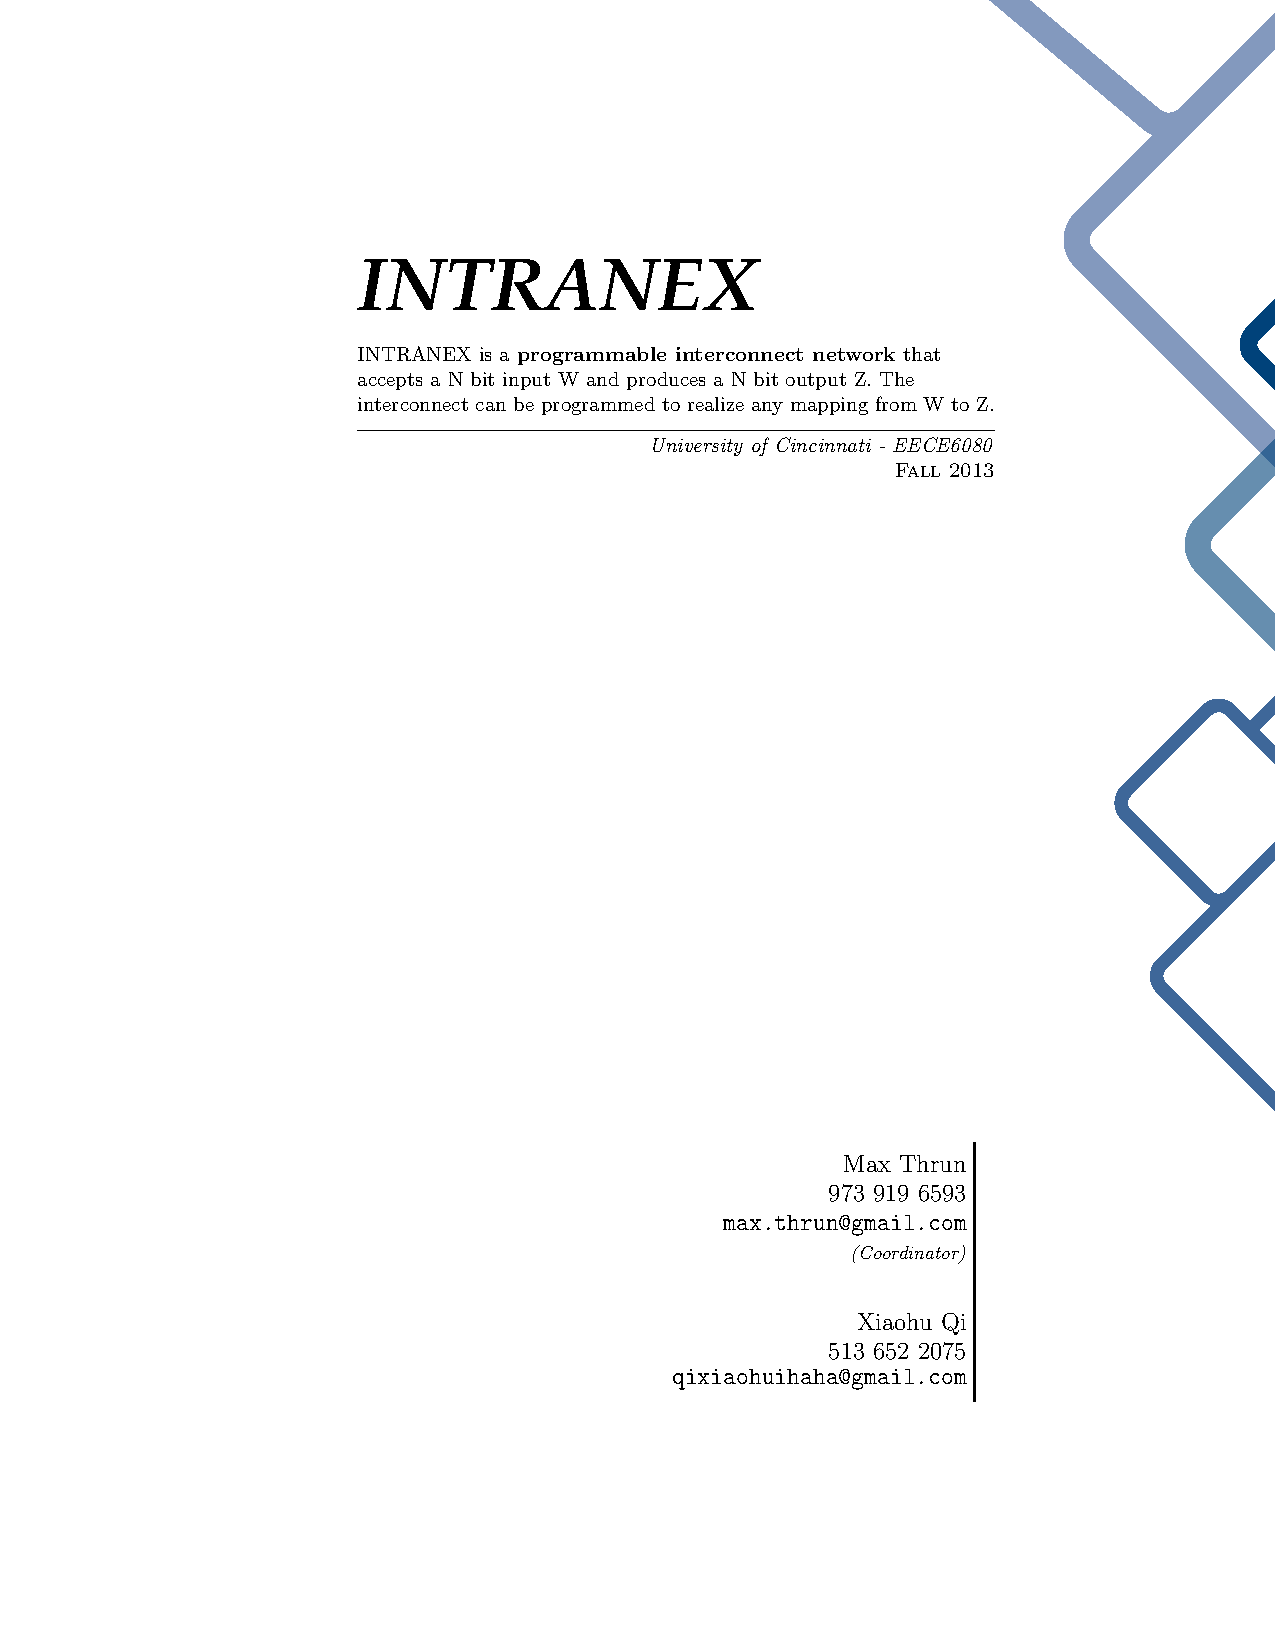
\includepdf{../cover_page/cover_page.pdf}
\parskip = 0.2\baselineskip
\newpage
\tableofcontents
\newpage
\listoffigures
\listoftables
\lstlistoflistings
\parskip = 0.5\baselineskip
\newpage
\section{Pinout Diagram}

The pinout diagram for INTRANEX is shown below in Figure~\ref{fig:pinout}.
Pins that are currently unutilized will be assigned to various internal logic
signals once the floorplan is finalized. Note the symmetry of the core
functionality.  This was done so that multiple INTRANEX chip can be directly
chained together with minimal routing effort during PCB layout.

\begin{figure}[H]
    \centering
    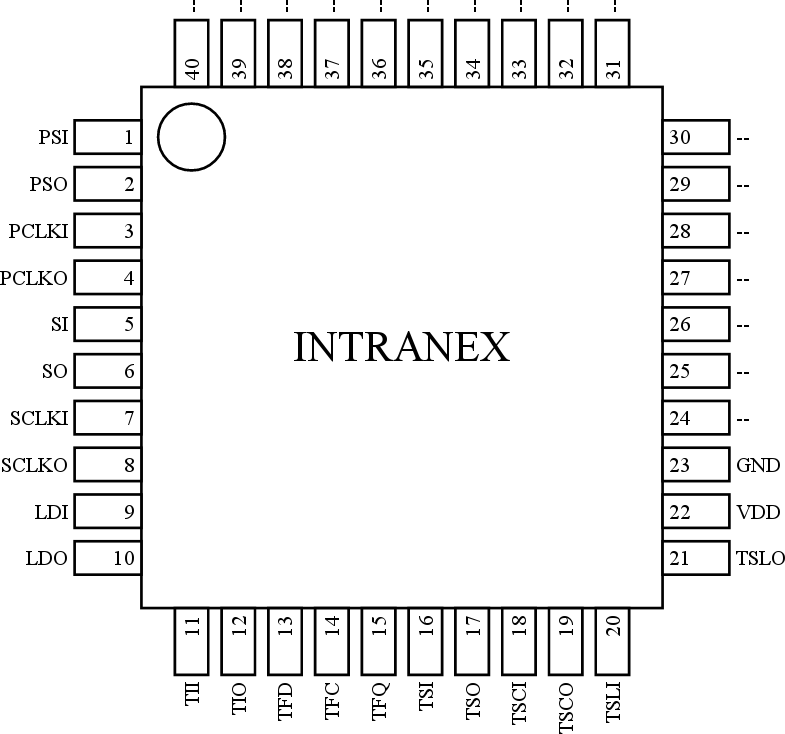
\includegraphics[width=\linewidth]{../pinout/pinout.png}
    \caption{Pinout Diagram}
    \label{fig:pinout}
\end{figure}

\newpage
The table below shows each pin and its corresponding name, type, and a brief
description of its functionality. Type is of either I (Input), O (Output), or P
(Power).
\begin{table}[H]
    \begin{tabularx}{\textwidth}{|l|l|c|X|}
        \hline
        \textbf{Pin \#} & \textbf{Name} & \textbf{Type} & \textbf{Description} \\
        \hline
        









%
%
%
%
%
%
%
%
%
%
% MAIN PINS
% TEST DFF
% TEST INVERTER
% TEST PIN SLICE
% TEST SHIFT SLICE
1  & TPZO   & O & Test pin slice row output \\ \hline
2  & TPZI   & I & Test pin slice row input \\ \hline
3 & TII   & I & Test inverter input \\ \hline
4 & TIO   & O & Test interter output \\ \hline
5  & PCLKI & I & PIN clock input \\ \hline
6  & PSI   & I & PIN serial input \\ \hline
7  & TESTI & I & Test Mode enable input\\ \hline
8  & SI    & I & Serial input \\ \hline
9  & LDI   & I & Parallel load input \\ \hline
10 & SCLKI & I & Serial clock input \\ \hline
11 & W0 & O & W0 Debug Output \\ \hline
12 & W1 & O & W0 Debug Output \\ \hline
13 & W2 & O & W0 Debug Output \\ \hline
14 & W3 & O & W0 Debug Output \\ \hline
15 & W4 & O & W0 Debug Output \\ \hline
16 & GND   & P & -- \\ \hline
17 & W12 & O & W0 Debug Output \\ \hline
18 & W13 & O & W0 Debug Output \\ \hline
19 & W14 & O & W0 Debug Output \\ \hline
20 & W15 & O & W0 Debug Output \\ \hline
21 & SCLKO & O & Serial clock output \\ \hline
22 & LDO   & O & Parallel load output \\ \hline
23 & SO    & O & Serial output \\ \hline
24 & TESTO & O & Test Mode enable output\\ \hline
25 & PSO   & O & PIN serial output \\ \hline
26 & PCLKO & O & PIN clock output \\ \hline
28 & TFQ   & O & Test flop-flop Q output \\ \hline
29 & TFC   & I & Test flip-flop clock input \\ \hline
30 & TFD   & I & Test flip-flop D input \\ \hline
31 & TSSO  & O & Test shift slice serial output \\ \hline
32 & TSZ   & I & Test shift slice parallel input \\ \hline
33 & TSSI  & I & Test shift slice serial input \\ \hline
34 & TSLI  & I & Test shift slice load input \\ \hline
35 & TSCI  & I & Test shift slice clock input \\ \hline
36 & VDD   & P & -- \\ \hline
37 & TPWI   & I & Test pin slice coloumn \\ \hline
38 & TPQO   & O & Test pin slice serial output \\ \hline
39 & TPQI   & I & Test pin slice serial input \\ \hline
40 & TPCI   & I & Test pin slice clock input \\ \hline

    \end{tabularx}
    \caption{Pin Descriptions}
\end{table}

\newpage
\section{Chip Functionality}

The major function of this chip is to take an N bit input and translate any bit
position to any other position. This allows for commonly desired functionality
such as bit reversing or nibble swapping. To accomplish this we use a N by N
bit interconnect network known as the PIN (Programmable Interconnect Network).
The PIN is configured to perform the desired bit mappings by clocking in the
mappings using the \texttt{PSI} (PIN Shift Input) and \texttt{PCLKI} (PIN Clock
Input) pins.  The value to be manipulated, called  the Input Value, Shift Value
or Shifter Value, is then clocked in serially using the \texttt{SI} (Shifter
Input) and \texttt{SCLKI} (Shifter Clock Input) pins. To obtain the result the
\texttt{LDI} (Load Input) pin is pulled high and the \texttt{SCLKI} pin is
pulsed to latch the result in to the shift register. Once the result is latched
the \texttt{LDI} pin is de-asserted and the result can be clocked out of the
\texttt{SO} (Shifter Output) pin. Note that the input value is clocked in MSB
first and the output value is clocked out MSB first as well.

\subsection{Configuring the Programmable Interconnect Network}

A timing diagram illustrating the PIN configuration process for a 3-Bit
INTRANEX is shown below. For a 3-Bit input value a 3x3 grid is required
resulting in a PIN configuration vector of 9 Bits. The mapping for each of
these bits is also labels and will be explained further in later sections.

\begin{figure}[H]
    \centering
    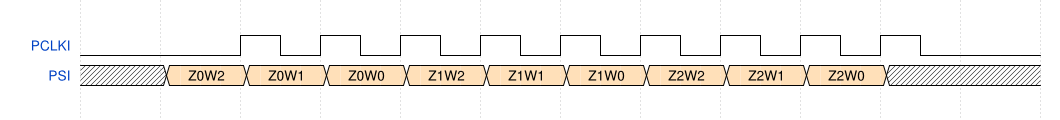
\includegraphics[width=\linewidth]{../waveforms/pin.png}
    \caption{PIN Configuration}
\end{figure}

\subsection{Loading and reading a value}

Loading an input value is achieved by clocking the value in on the \texttt{SI}
pin using the \texttt{SCLKI} pin. The \texttt{LDI} pin must be held low during
this operation. The diagram below illustrates this process and shows the bit
definitions of the value being clocked in.

\begin{figure}[H]
    \centering
    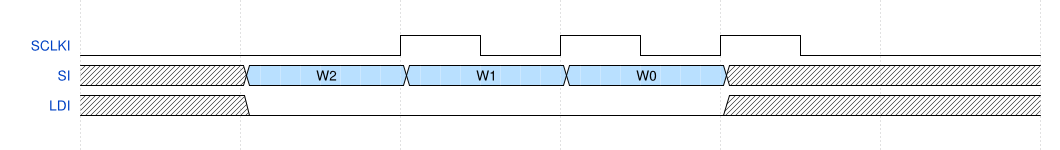
\includegraphics[width=\linewidth]{../waveforms/shift_load.png}
    \caption{Loading a value}
\end{figure}

After the value has been loaded in the result is clocked on in a similar
fashion. To first latch the result the \texttt{LDI} pin needs to be held high
and the \texttt{SCLKI} pin pulsed. The MSB of the result is now available on
the \texttt{SO}. The \texttt{LDI} pin should now be held low while clocking out
the remaining result bits.

\begin{figure}[H]
    \centering
    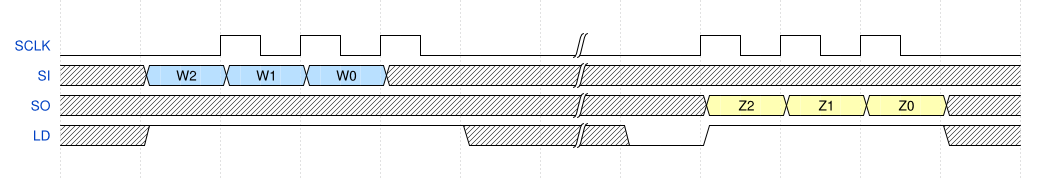
\includegraphics[width=\linewidth]{../waveforms/shift_load_read.png}
    \caption{Loading a value and reading the result}
\end{figure}

\subsection{Test Mode}

Test Mode is enabled by pulling the \texttt{TESTI} pin high. When this occurs
the output of the internal shift register is rerouted to connect to the input
of the PIN network bypassing its normal \texttt{PSI} input.  Additionally the
\texttt{SCLKO} signal is also routed to the PIN bypassing its normal
\texttt{PCLKI} signal. Finally the \texttt{PSO} signal is routed to the
\texttt{SO} pin. This allows values that are clocked in via the \texttt{SI} pin
to propagate through the shifter and then through the PIN and then out the
\texttt{SO} pin. The fact that the values come out the \texttt{SO} pin allows
multiple INTRANEX chips to be directly chained and tested in circuit using only the
\texttt{SI} and \texttt{SCLKI} pins of the first chip in the chain. Note that
the \texttt{LDI} pin must be held low during this entire operation in order to
ensure proper shifting through the shift register.

\begin{figure}[H]
    \centering
    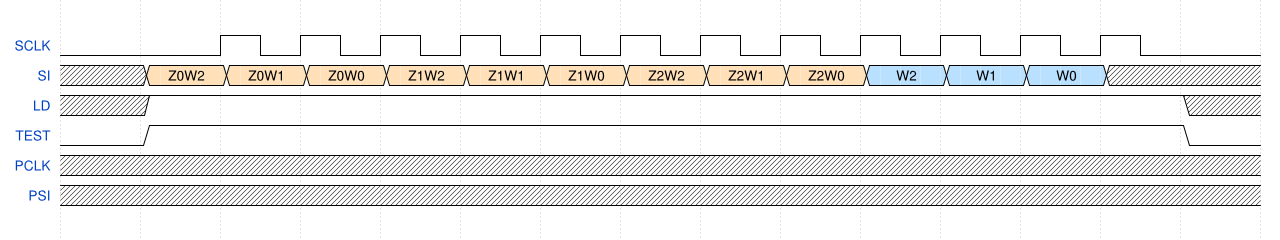
\includegraphics[width=\linewidth]{../waveforms/test.png}
    \caption{Enabling test mode and loading all DFFs}
\end{figure}

\section{Design Decisions}

When evaluating design concepts and possible solutions we prioritized a few key
factors that we wanted to achieve. The first is a fully bit-sliced solution
where each slice can directly connect to the next with minimal wiring overhead
and zero additional logic. This will allow us to utilize Magics \texttt{Array}
functionality to quickly build up our chip and allow us to easily scale to any
desired size. As we see in later sections we were able to achieve a fully
bit-sliced design with zero logic overhead.

In order to achieve totally minimized wiring overhead it would be necessary to
design two different slice layouts, one of which is mirrored and flipped. This
would allow each row in the PIN to share a power rail with the adjacent row and
also minimize the length of the row-to-row wiring. This design however greatly
increases the complexity of the VHDL design as wiring the rows together becomes
trickier. Additionally we would have to maintain two different versions of the
PIN slices. We decided to instead go with a design where all slices are exactly
identical and the interconnect between them is linear. This allows for easier
calculation of PIN configuration values as every row has the same index order.
The only real disadvantage to this design is that we will require long
interconnects between slices. We are assuming for now that even with the added
capacitance of these long interconnects we will still be able to achieve max
clock speeds of greater than 50Mhz. By progress report 2 we will have layout
simulation results to confirm this.

As stated earlier an important goal for use was to be able to directly chain
multiple INTRANEX chips together. Our current design achieves this and an
example chain showing 3 INTRANEXs chained together is shown below. Note that
the pin layout in this diagram matches that of the actual layout we plan on
implementing.

    \begin{figure}[H]
        \centering
        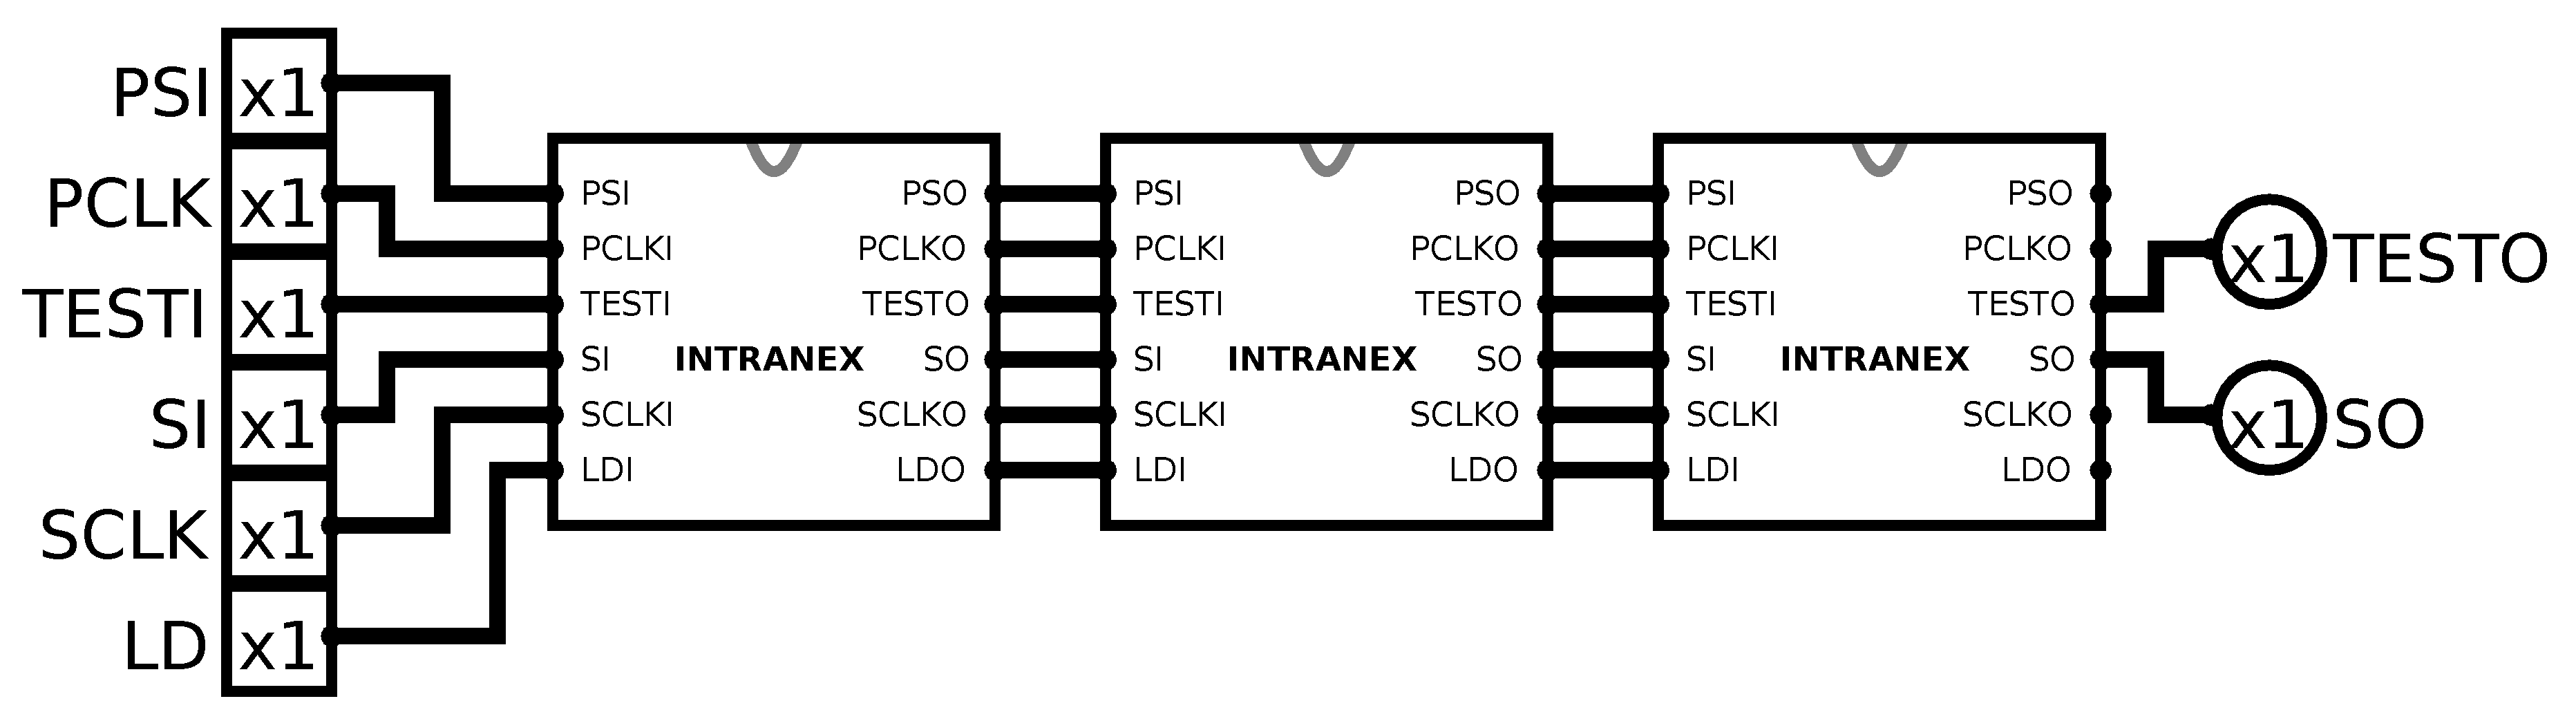
\includegraphics[width=\linewidth]{../../logisim/chain.png}
        \caption{3 INTRANEX Chain}
    \end{figure}

\section{Block Diagrams}

    \subsection{Top Level}
    A top level block diagram for a 3-bit INTRANEX is shown below. The top
    module is the PIN and the bottom module is the parallel load. Test mode
    logic has been excluded to illustrate only core functionality.
    \begin{figure}[H]
        \centering
        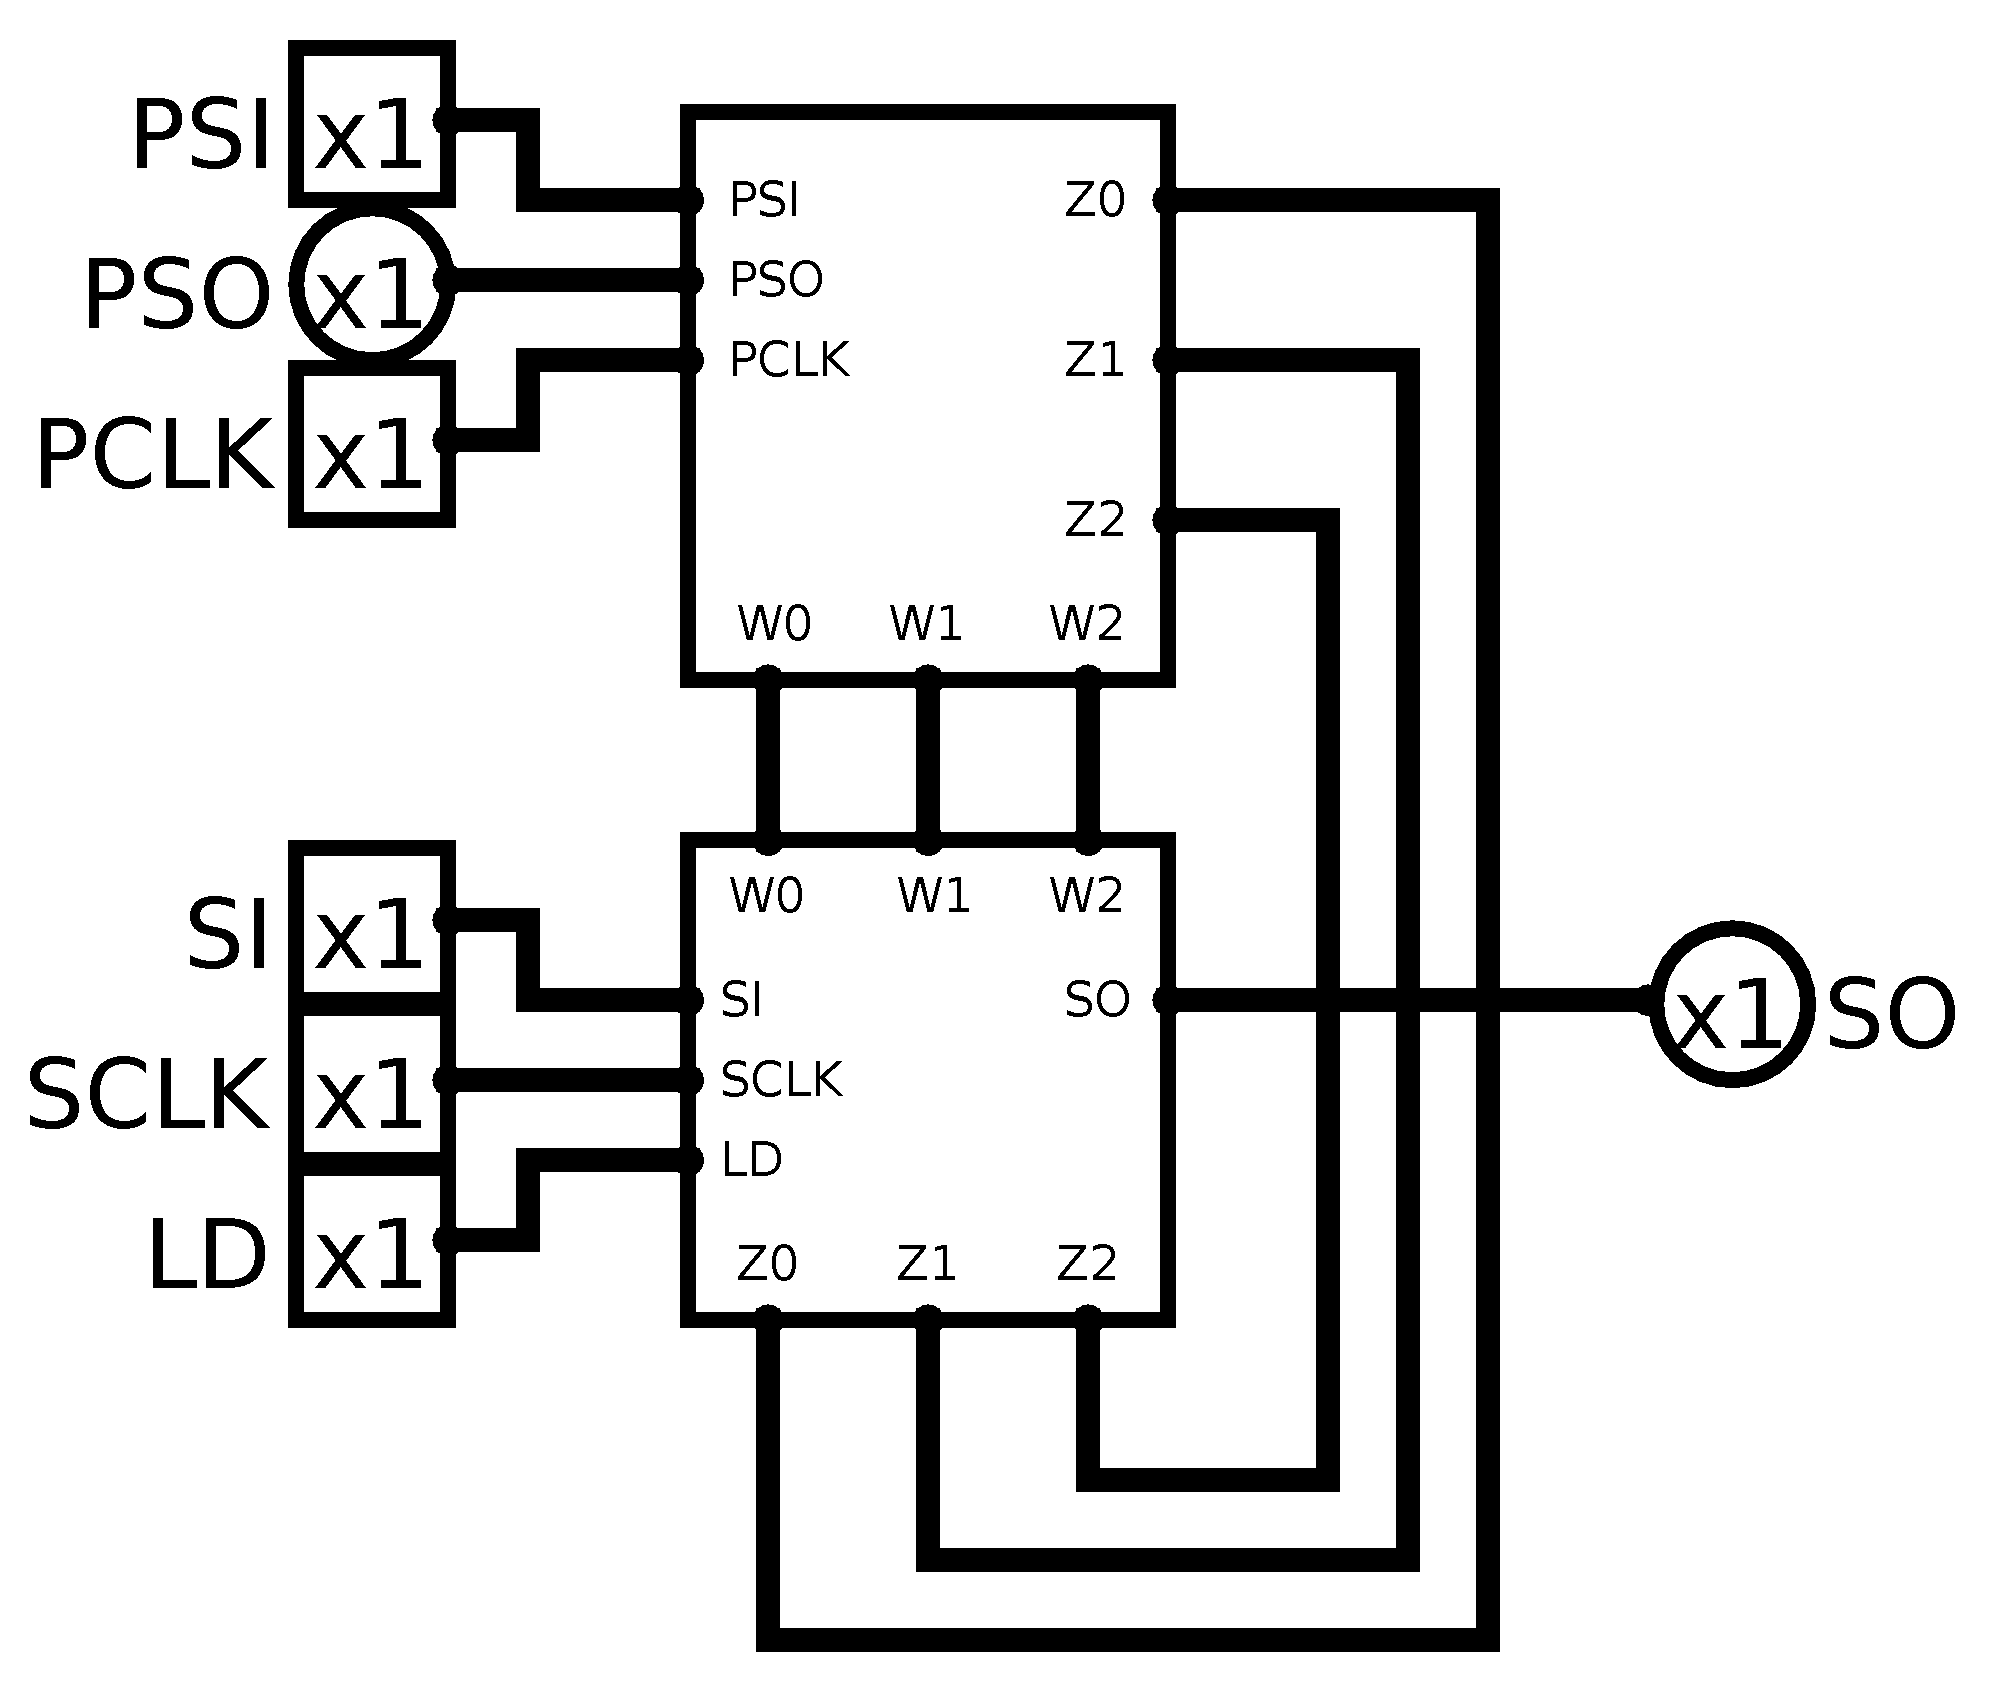
\includegraphics[width=0.75\linewidth]{../../logisim/top.png}
        \caption{Top Level Block Diagram (3-Bit Configuration)}
        \label{fig:block}
    \end{figure}

    \subsection{Top Level With Test Mode }
    The same top level diagram is shown below except this time with the test
    mode logic. The test mode logic simply consists of 3 2:1 multiplexers that
    redirect the output of the shift register to the input of the PIN and the
    output of the PIN to what is normally the output of the shift register. In
    other words, it wires in the PIN between the shifter and the shifters
    normal output pins.
    \begin{figure}[H]
        \centering
        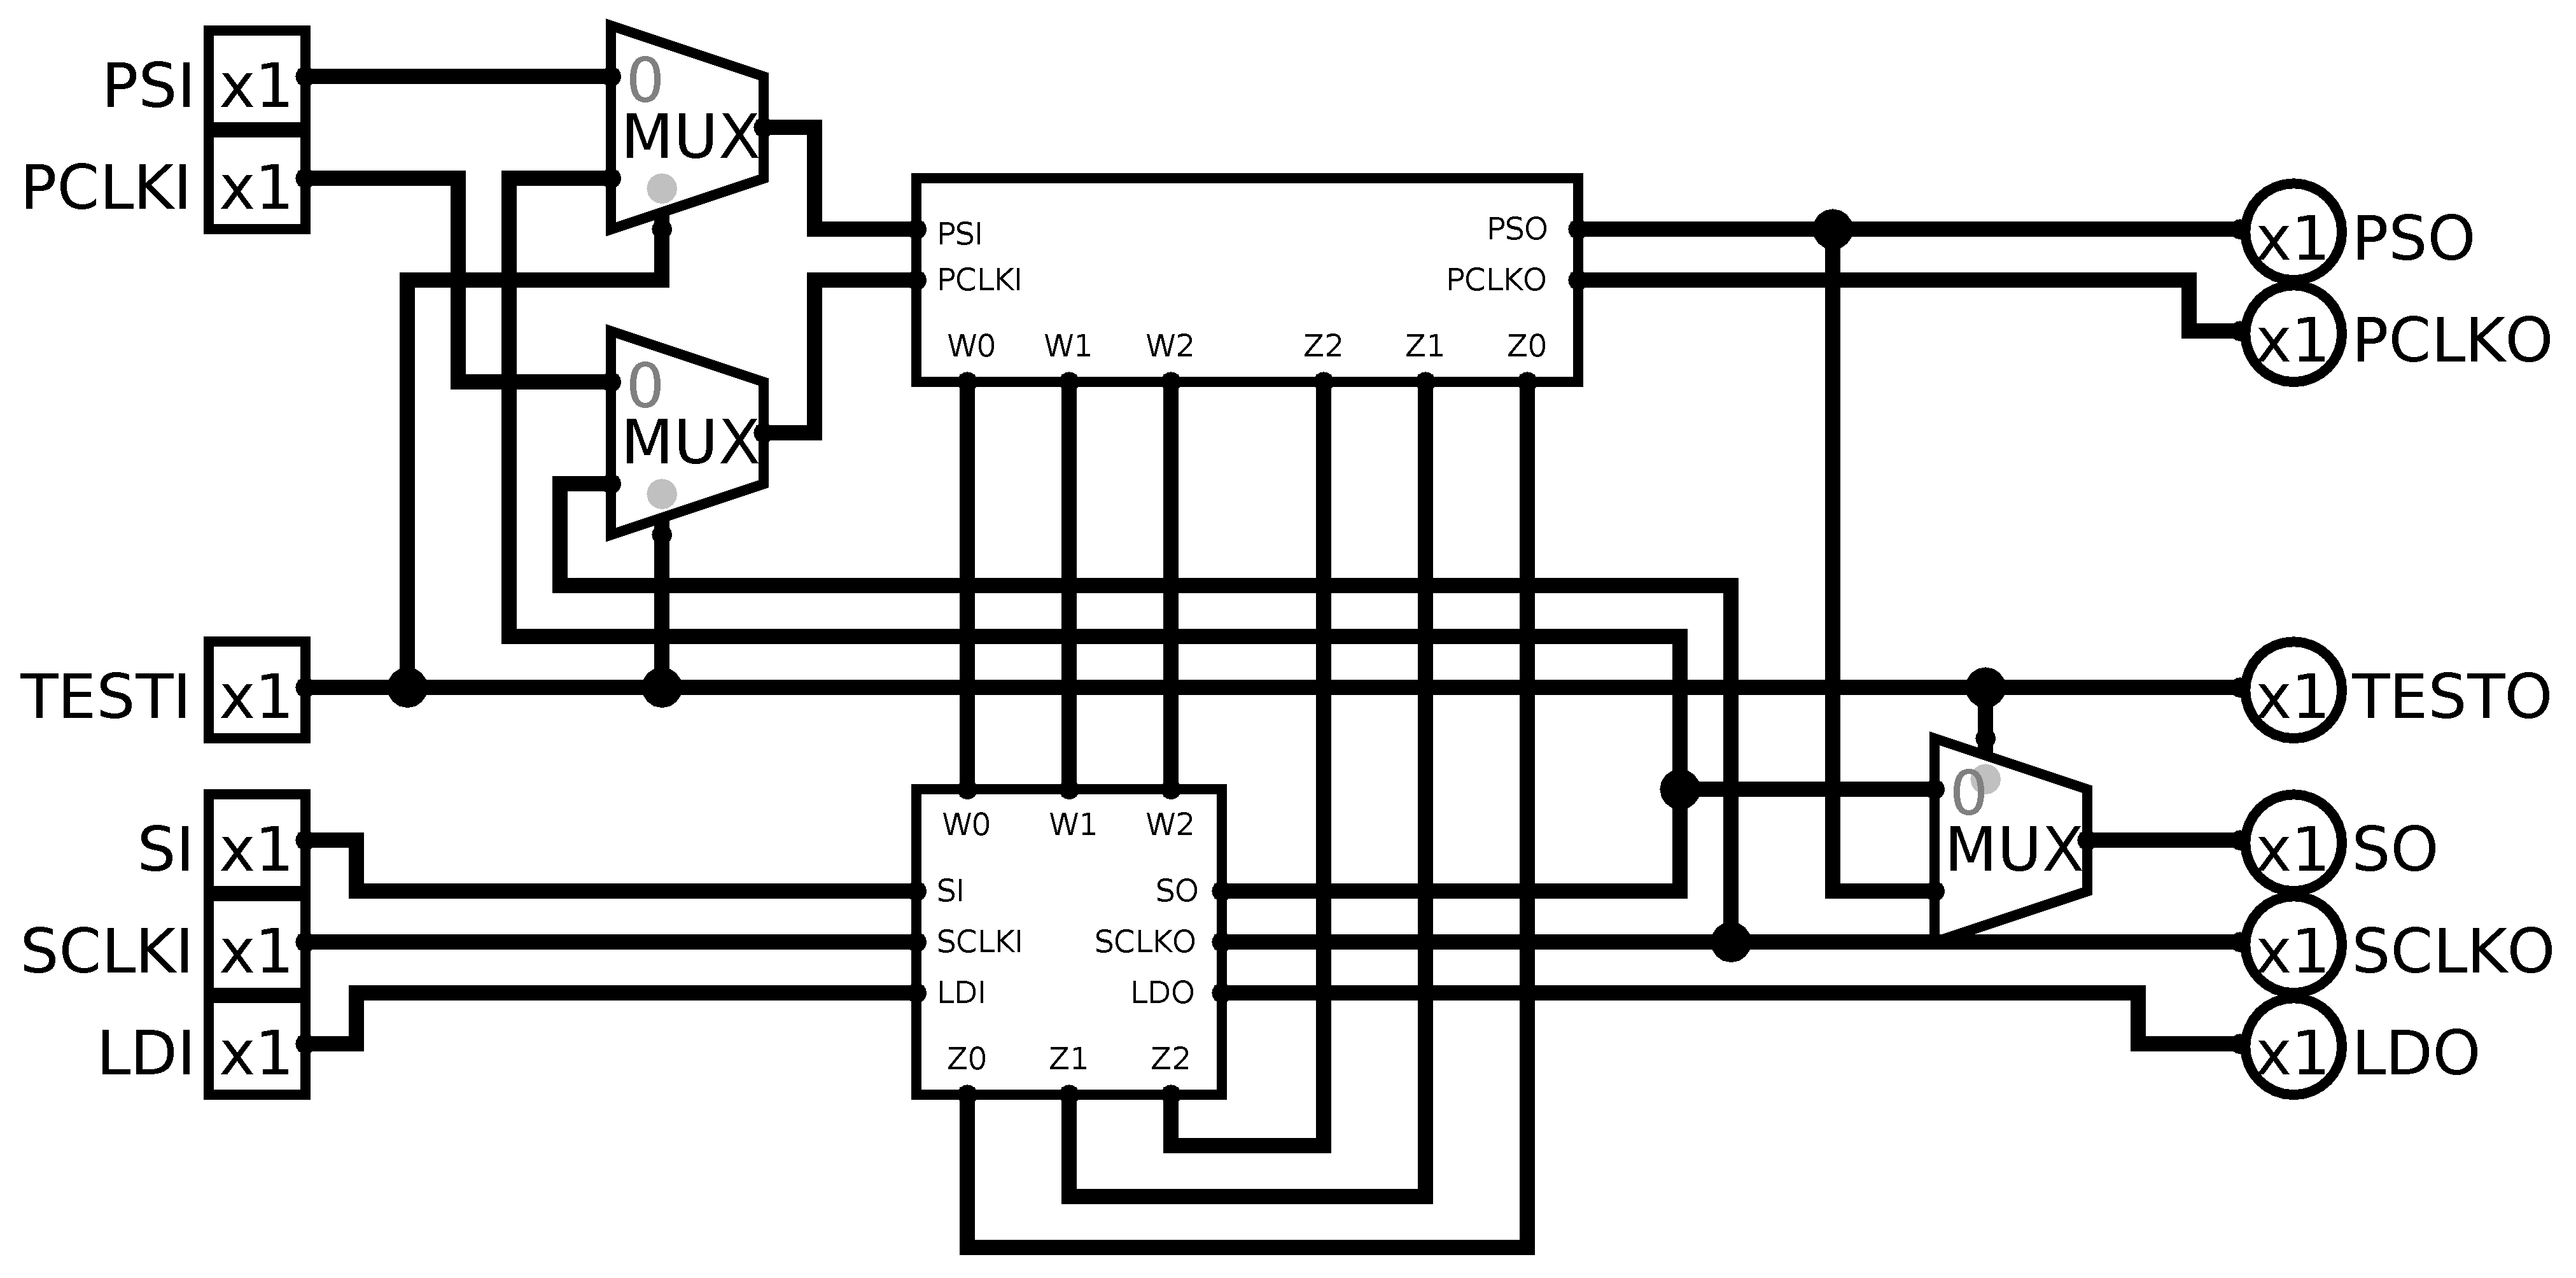
\includegraphics[width=0.9\linewidth]{../../logisim/test_mode.png}
        \caption{Top Level Block Diagram Showing Test Mode Logic (3-Bit Configuration)}
    \end{figure}

    \subsection{Top Level Bit Sliced}
    The diagram below shows a bit sliced version of Figure~\ref{fig:block}. We
    can see how each slice is directly connected together with zero interfacing
    logic.  We can also see the long row-to-row connections as discussed
    earlier.
    \vspace{2\baselineskip}
    \begin{figure}[H]
        \centering
        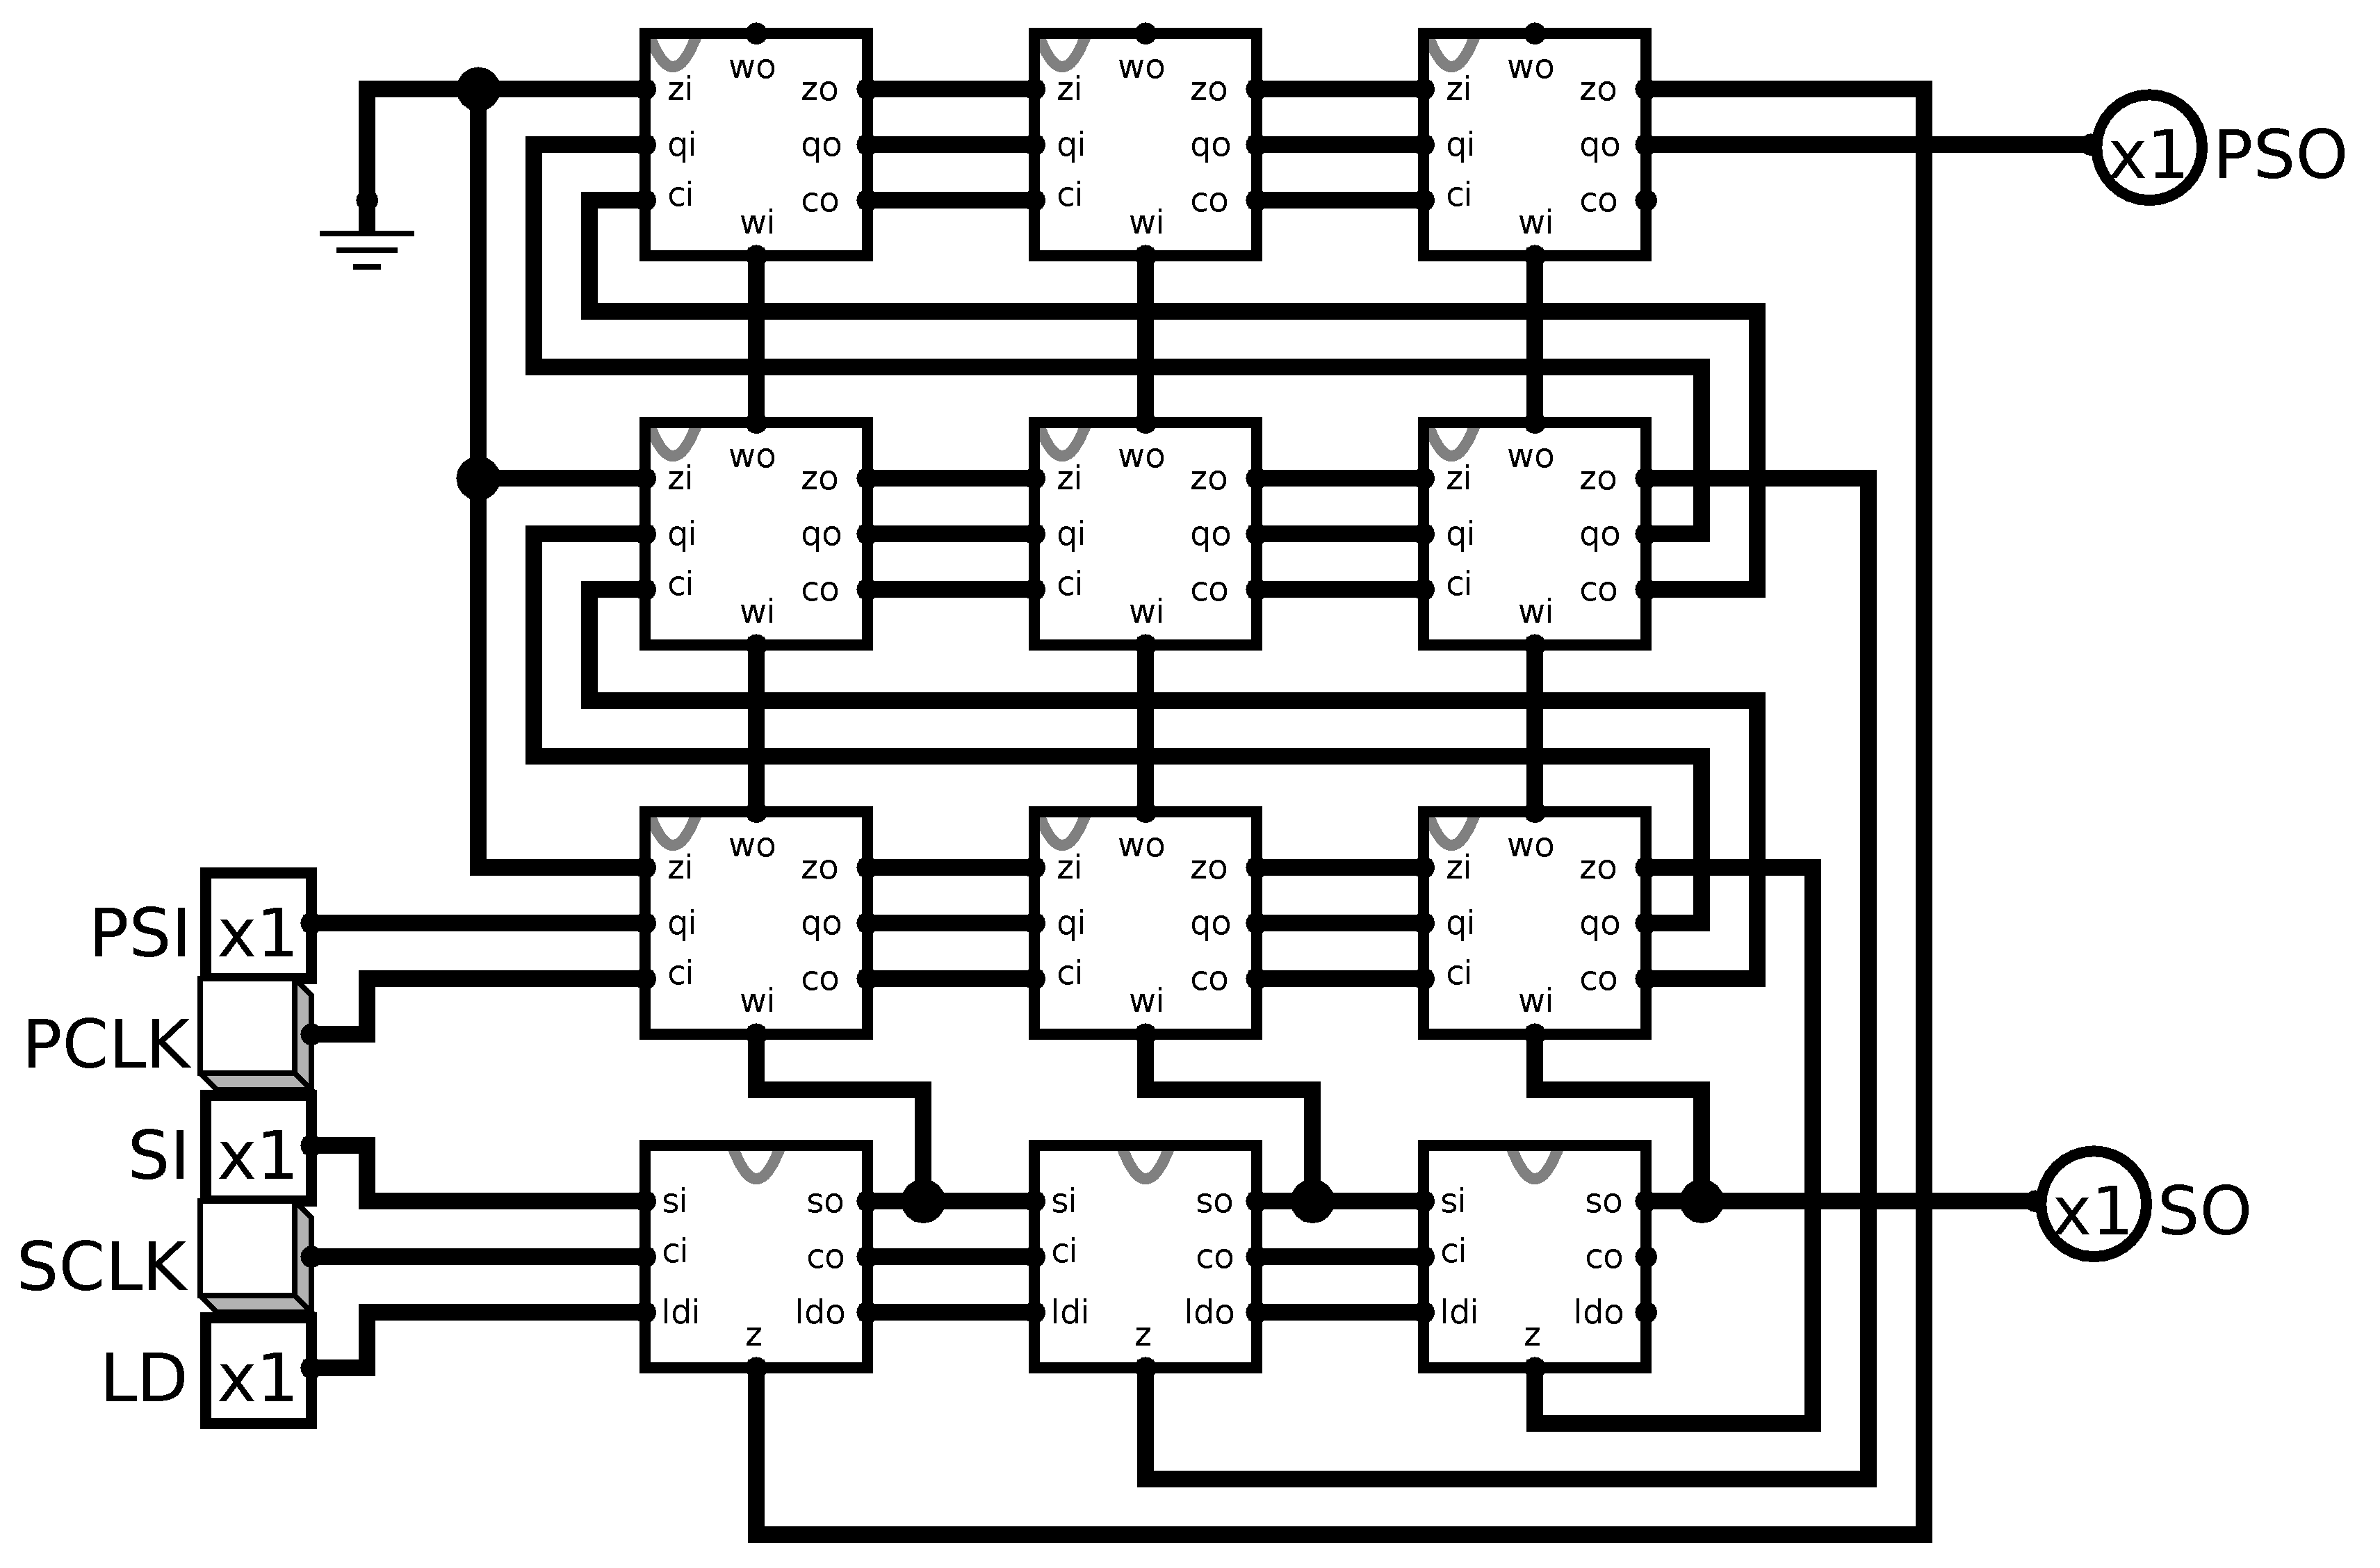
\includegraphics[width=\linewidth]{../../logisim/top_internal.png}
        \caption{Top Level Bit Sliced Block Diagram (3-Bit Configuration)}
    \end{figure}

    \newpage
    \subsection{Parallel Load Shift Register}

        \subsubsection{Bit-slicing Scheme}
        Looking at just the shift register we can see that it is a parallel
        load parallel output shifter that is easily extendable by simply
        tacking on additional slices.
        \begin{figure}[H]
            \centering
            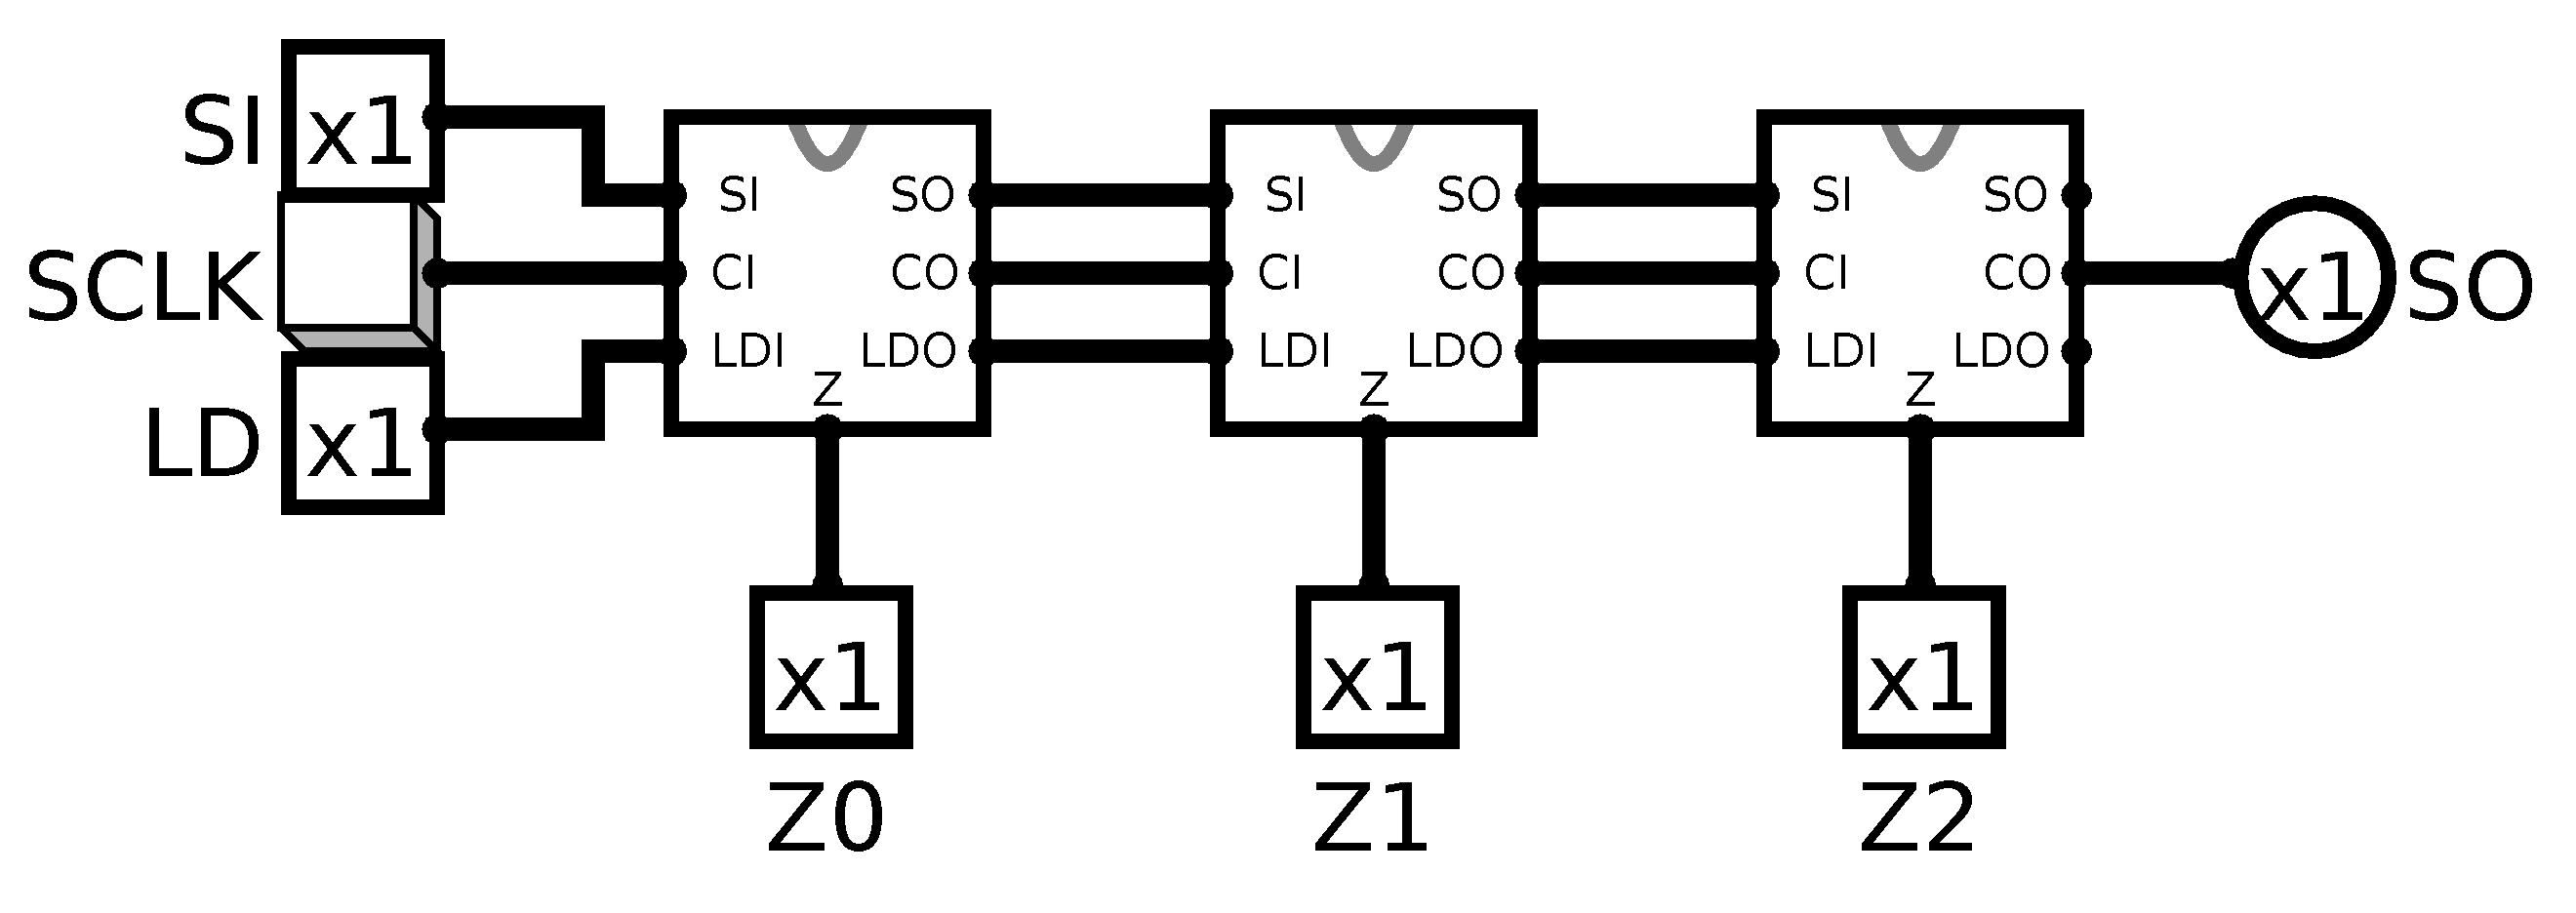
\includegraphics[width=\linewidth]{../../logisim/shift.png}
            \caption{Parallel Load Bit-Sliced Shifter Register (3-Bit Configuration)}
        \end{figure}

        \subsubsection{Bit-Slice}
        Looking at the internals of a single shift slice we can see that is is
        just a 2:1 multiplexer and a D Flip Flop. The multiplexer determines if
        the slice should load either the value from the previous slice
        (\texttt{SI}) or the parallel input (\texttt{Z}). When \texttt{LDI} is
        0 it uses the value of the previous slice and when it is a 1 it uses
        the parallel load value.
        \begin{figure}[H]
            \centering
            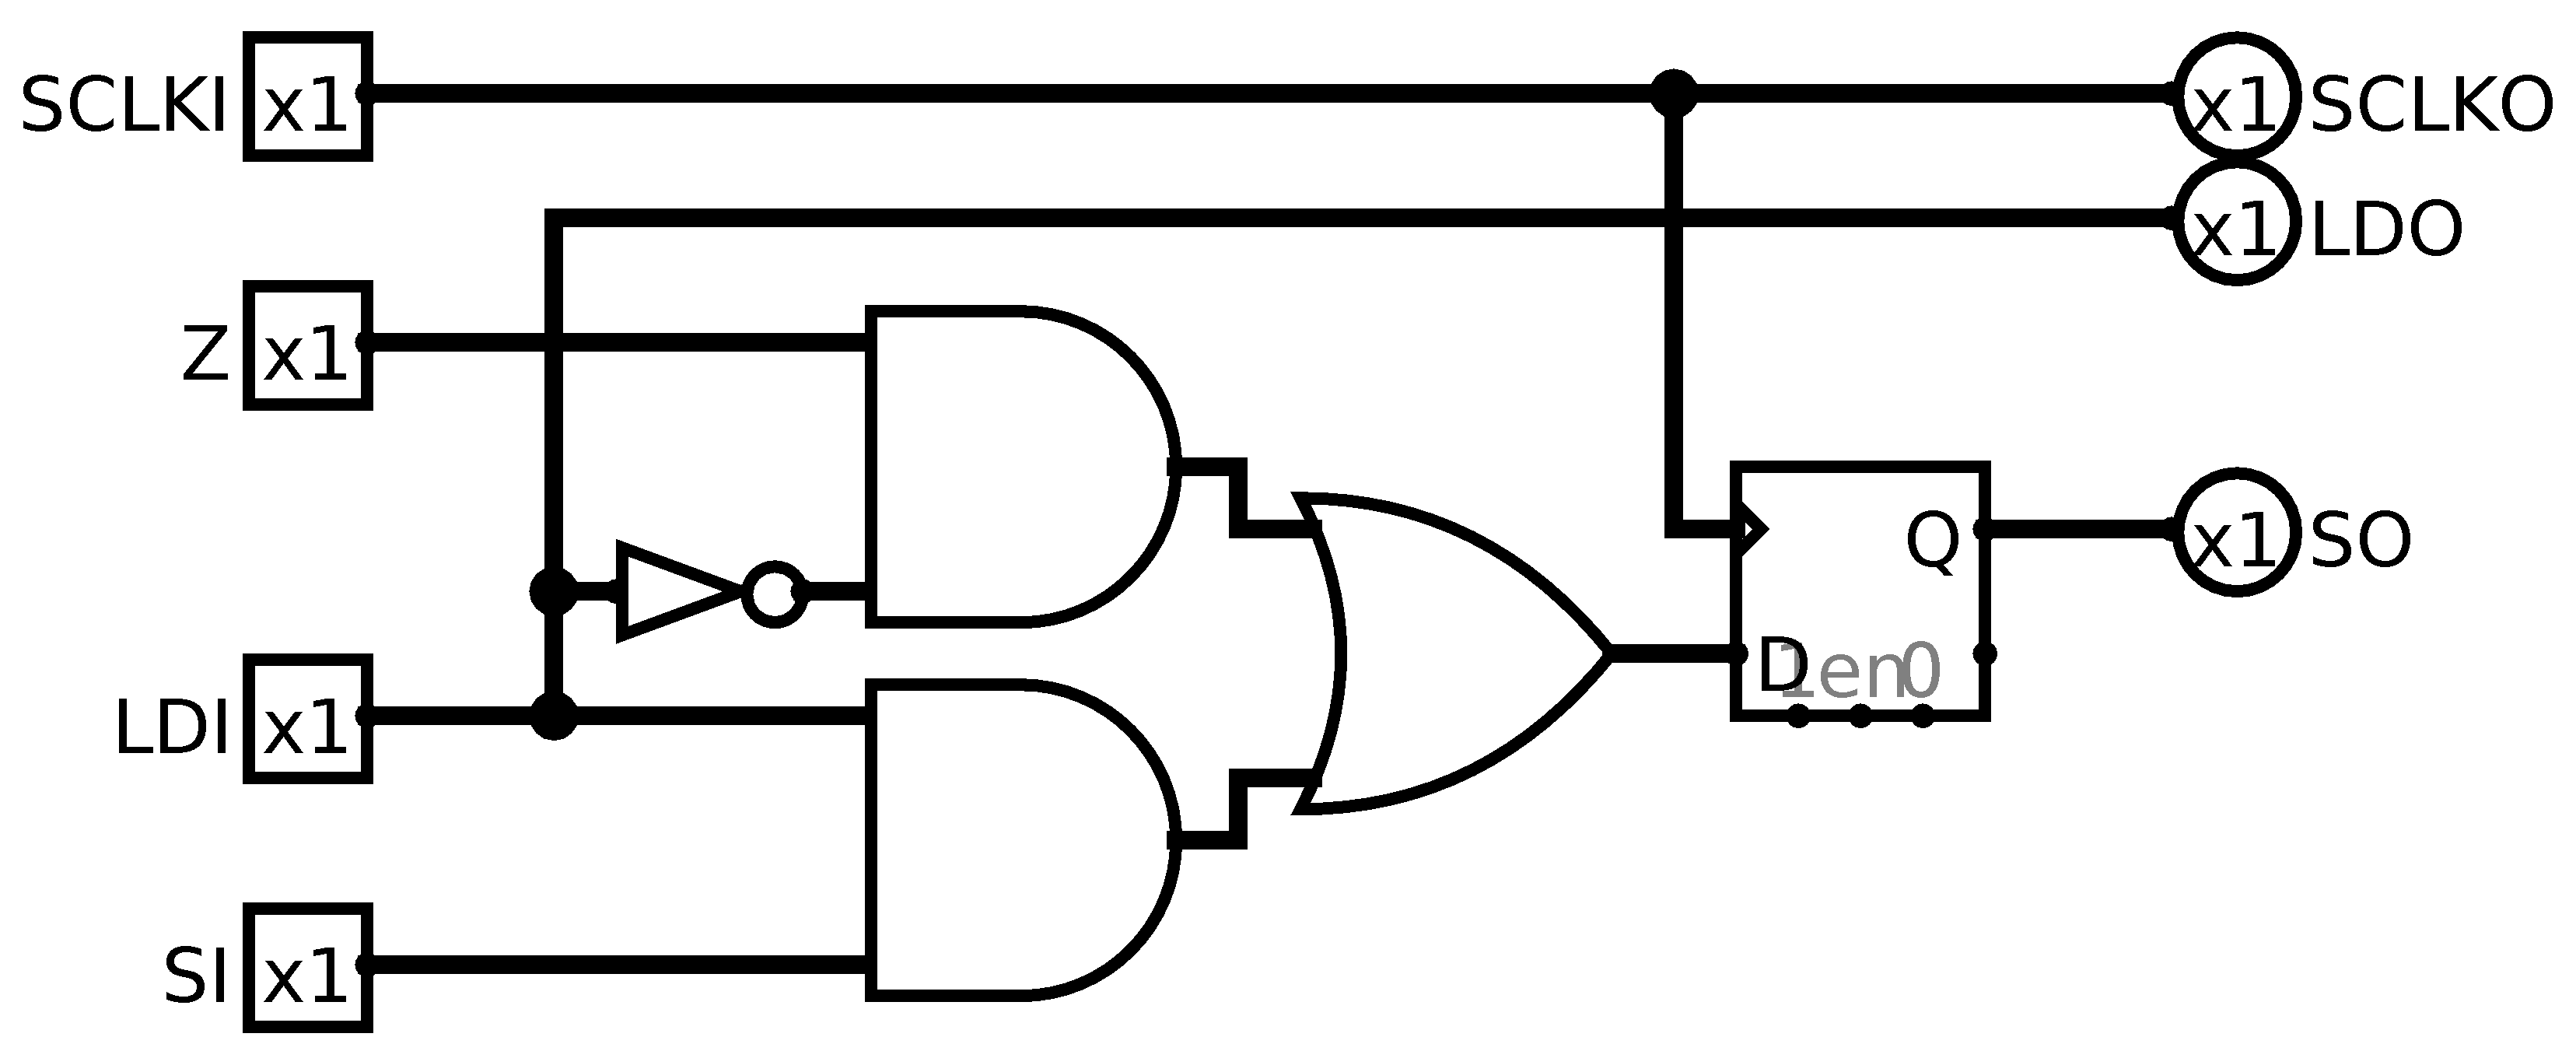
\includegraphics[width=\linewidth]{../../logisim/shift_slice.png}
            \caption{Parallel Load Shifter Register Bit-Slice}
        \end{figure}

    \newpage
    \subsection{Programmable Interconnect Network}

        \subsubsection{Bit-slicing Scheme}
        The diagram below showns just the PIN in bit-slice form. One of the
        design decisions made while determining the slice interconnects was to
        also pass the \texttt{PCLK} from slice to slice. The alternative was to
        simply connect each slices \texttt{PCLKI} to the main \texttt{PCLKI}
        pin at a higher level. We wanted to avoid as much manual layout as
        possible so it determined to be easier and cleaner to route the clock
        in such as way that it would be automatically connected when we layout
        the array.
        \begin{figure}[H]
            \centering
            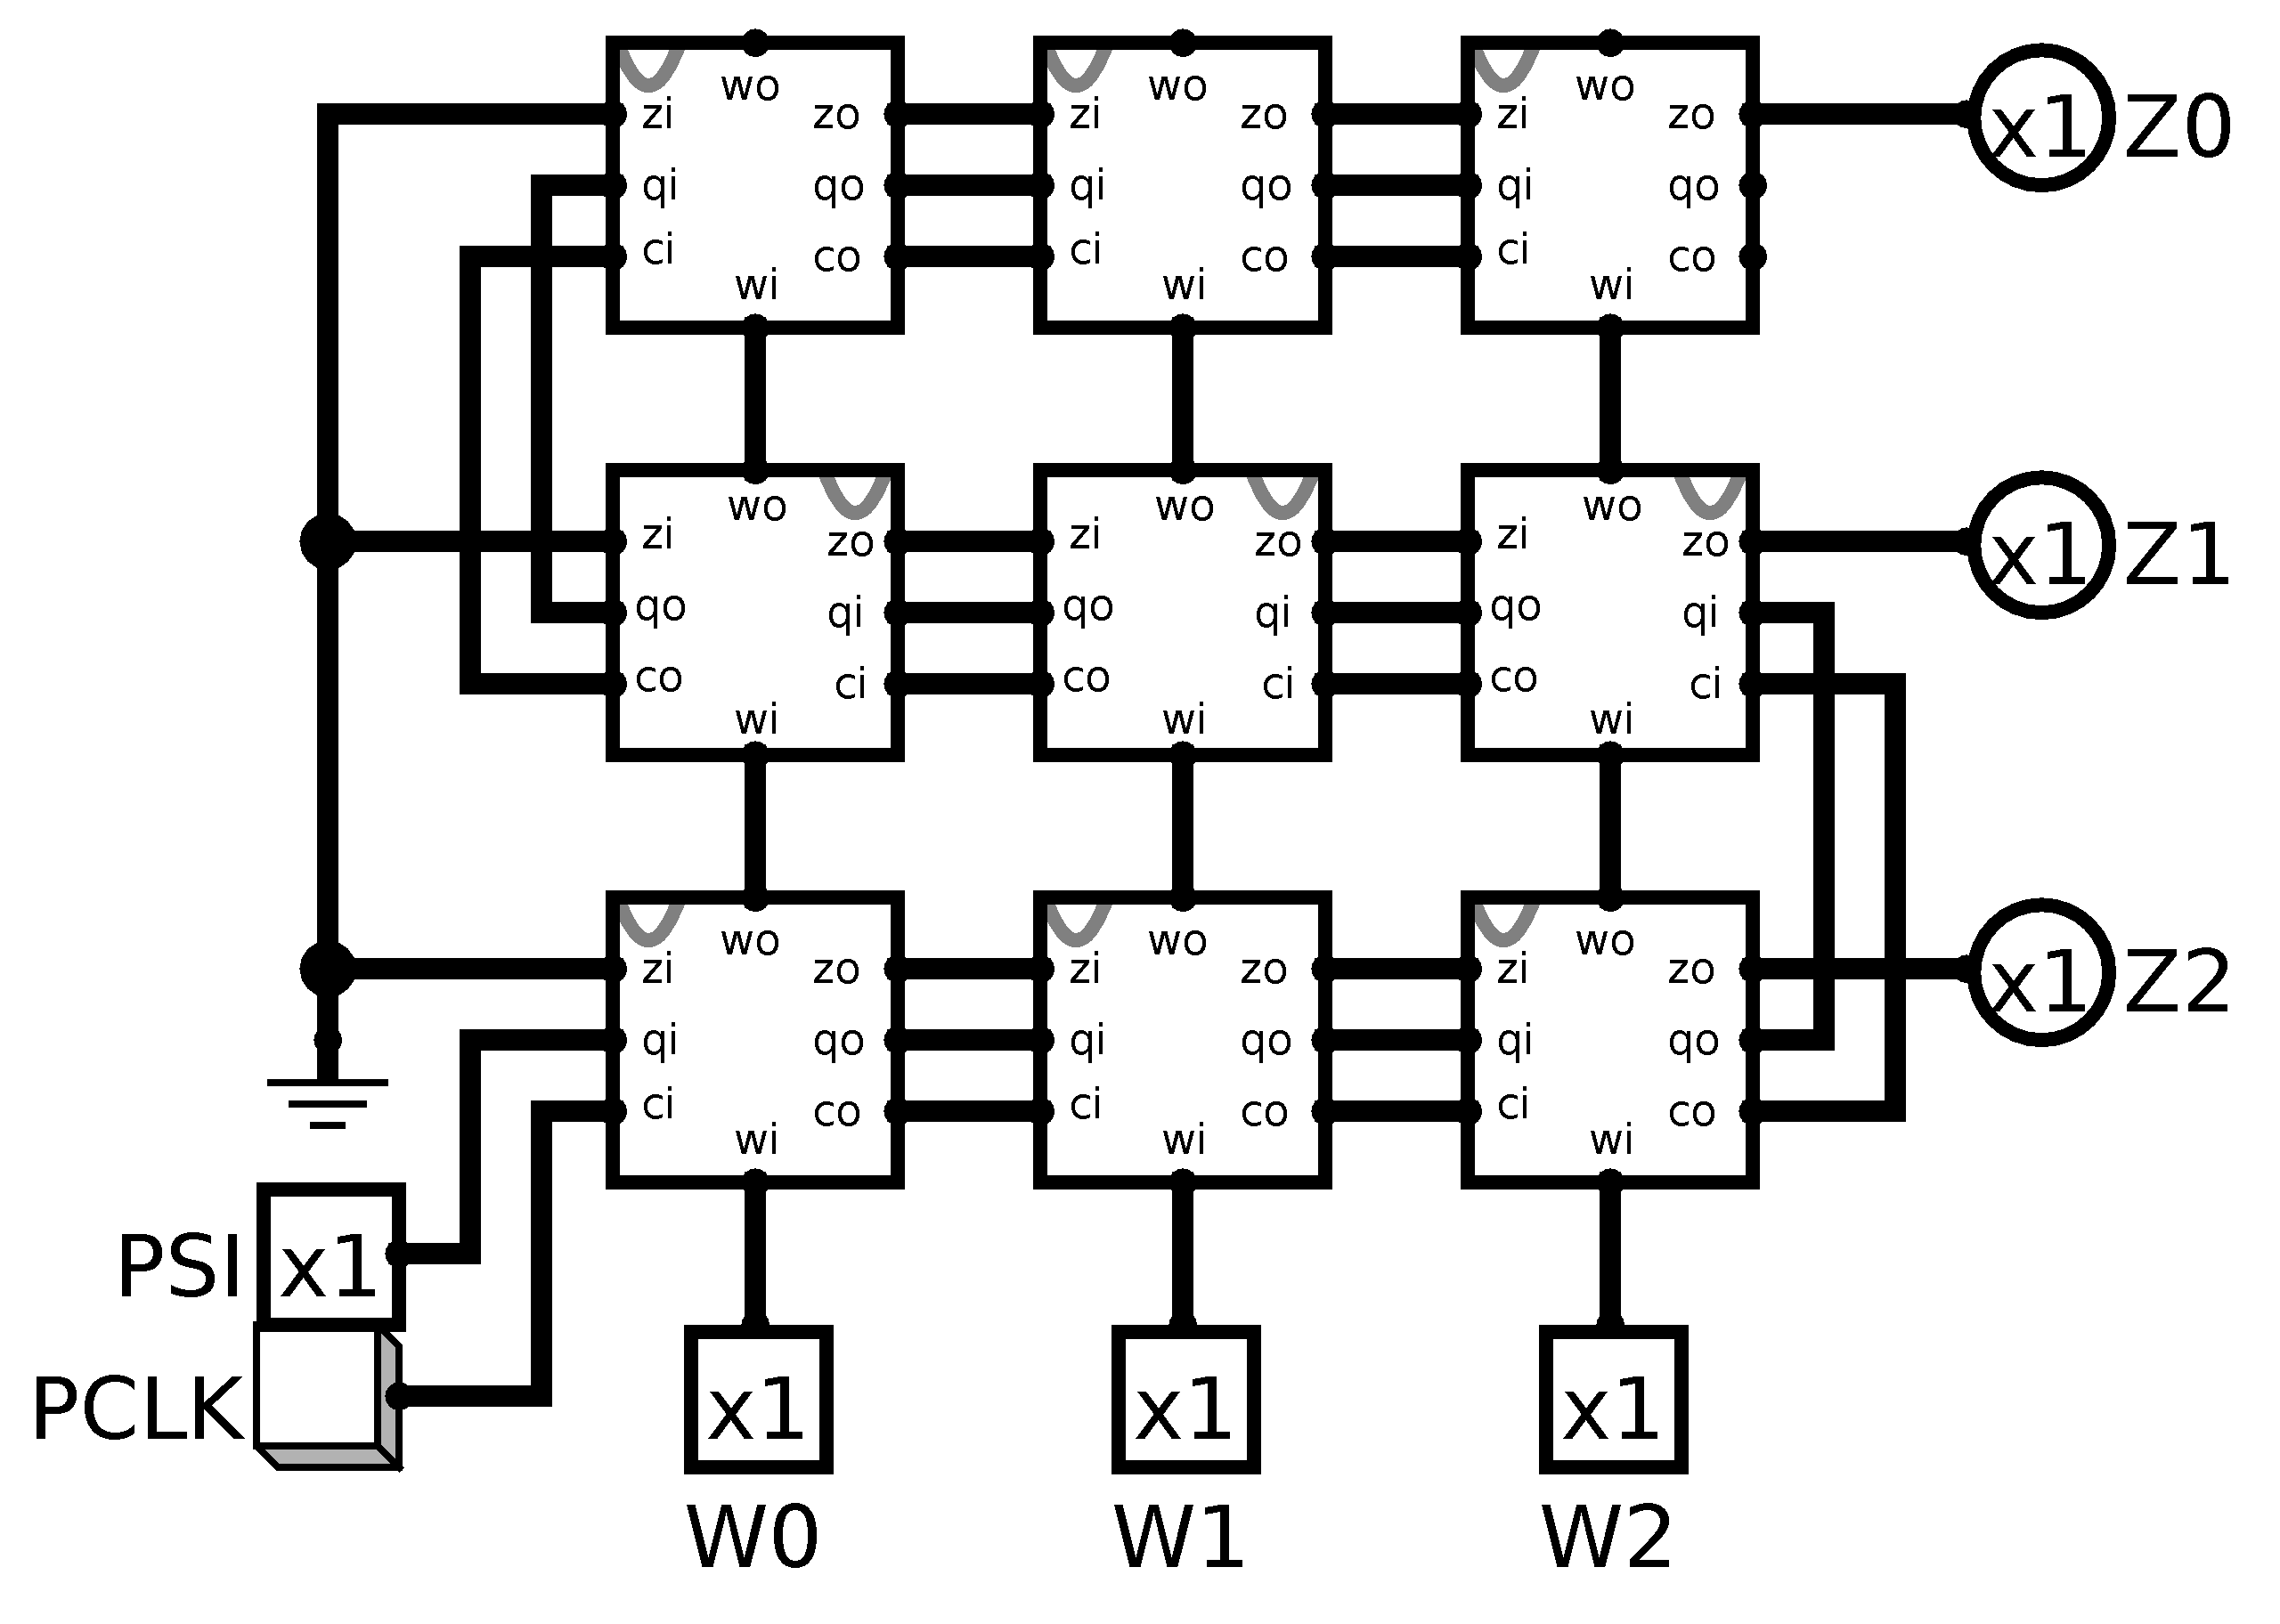
\includegraphics[width=0.5\linewidth]{../../logisim/pin.png}
            \caption{Bit-Sliced Programmable Interconnect Network (3-Bit Configuration)}
        \end{figure}

        \subsubsection{Bit-Slice}
        The PIN bit-slices, one of which is shown below, is what drive the
        whole functionality of our chip. \texttt{WI} is the input values bit
        for the current row. If that bit is set and this slice is configured as
        `connected' we want to output a logic high on the \texttt{Z} bus. We
        cannot, however, just simply \texttt{AND} these two values together and
        attach it to the bus as this would allow for multiple slices to drive
        or sink the bus. To avoid this we use an \texttt{OR} gate to determine
        if the slice behind us is outputting a 1. If so we just pass it along.
        If we want to output a 1 it is also no problem as the \texttt{OR} will
        accommodate us as well.
        \begin{figure}[H]
            \centering
            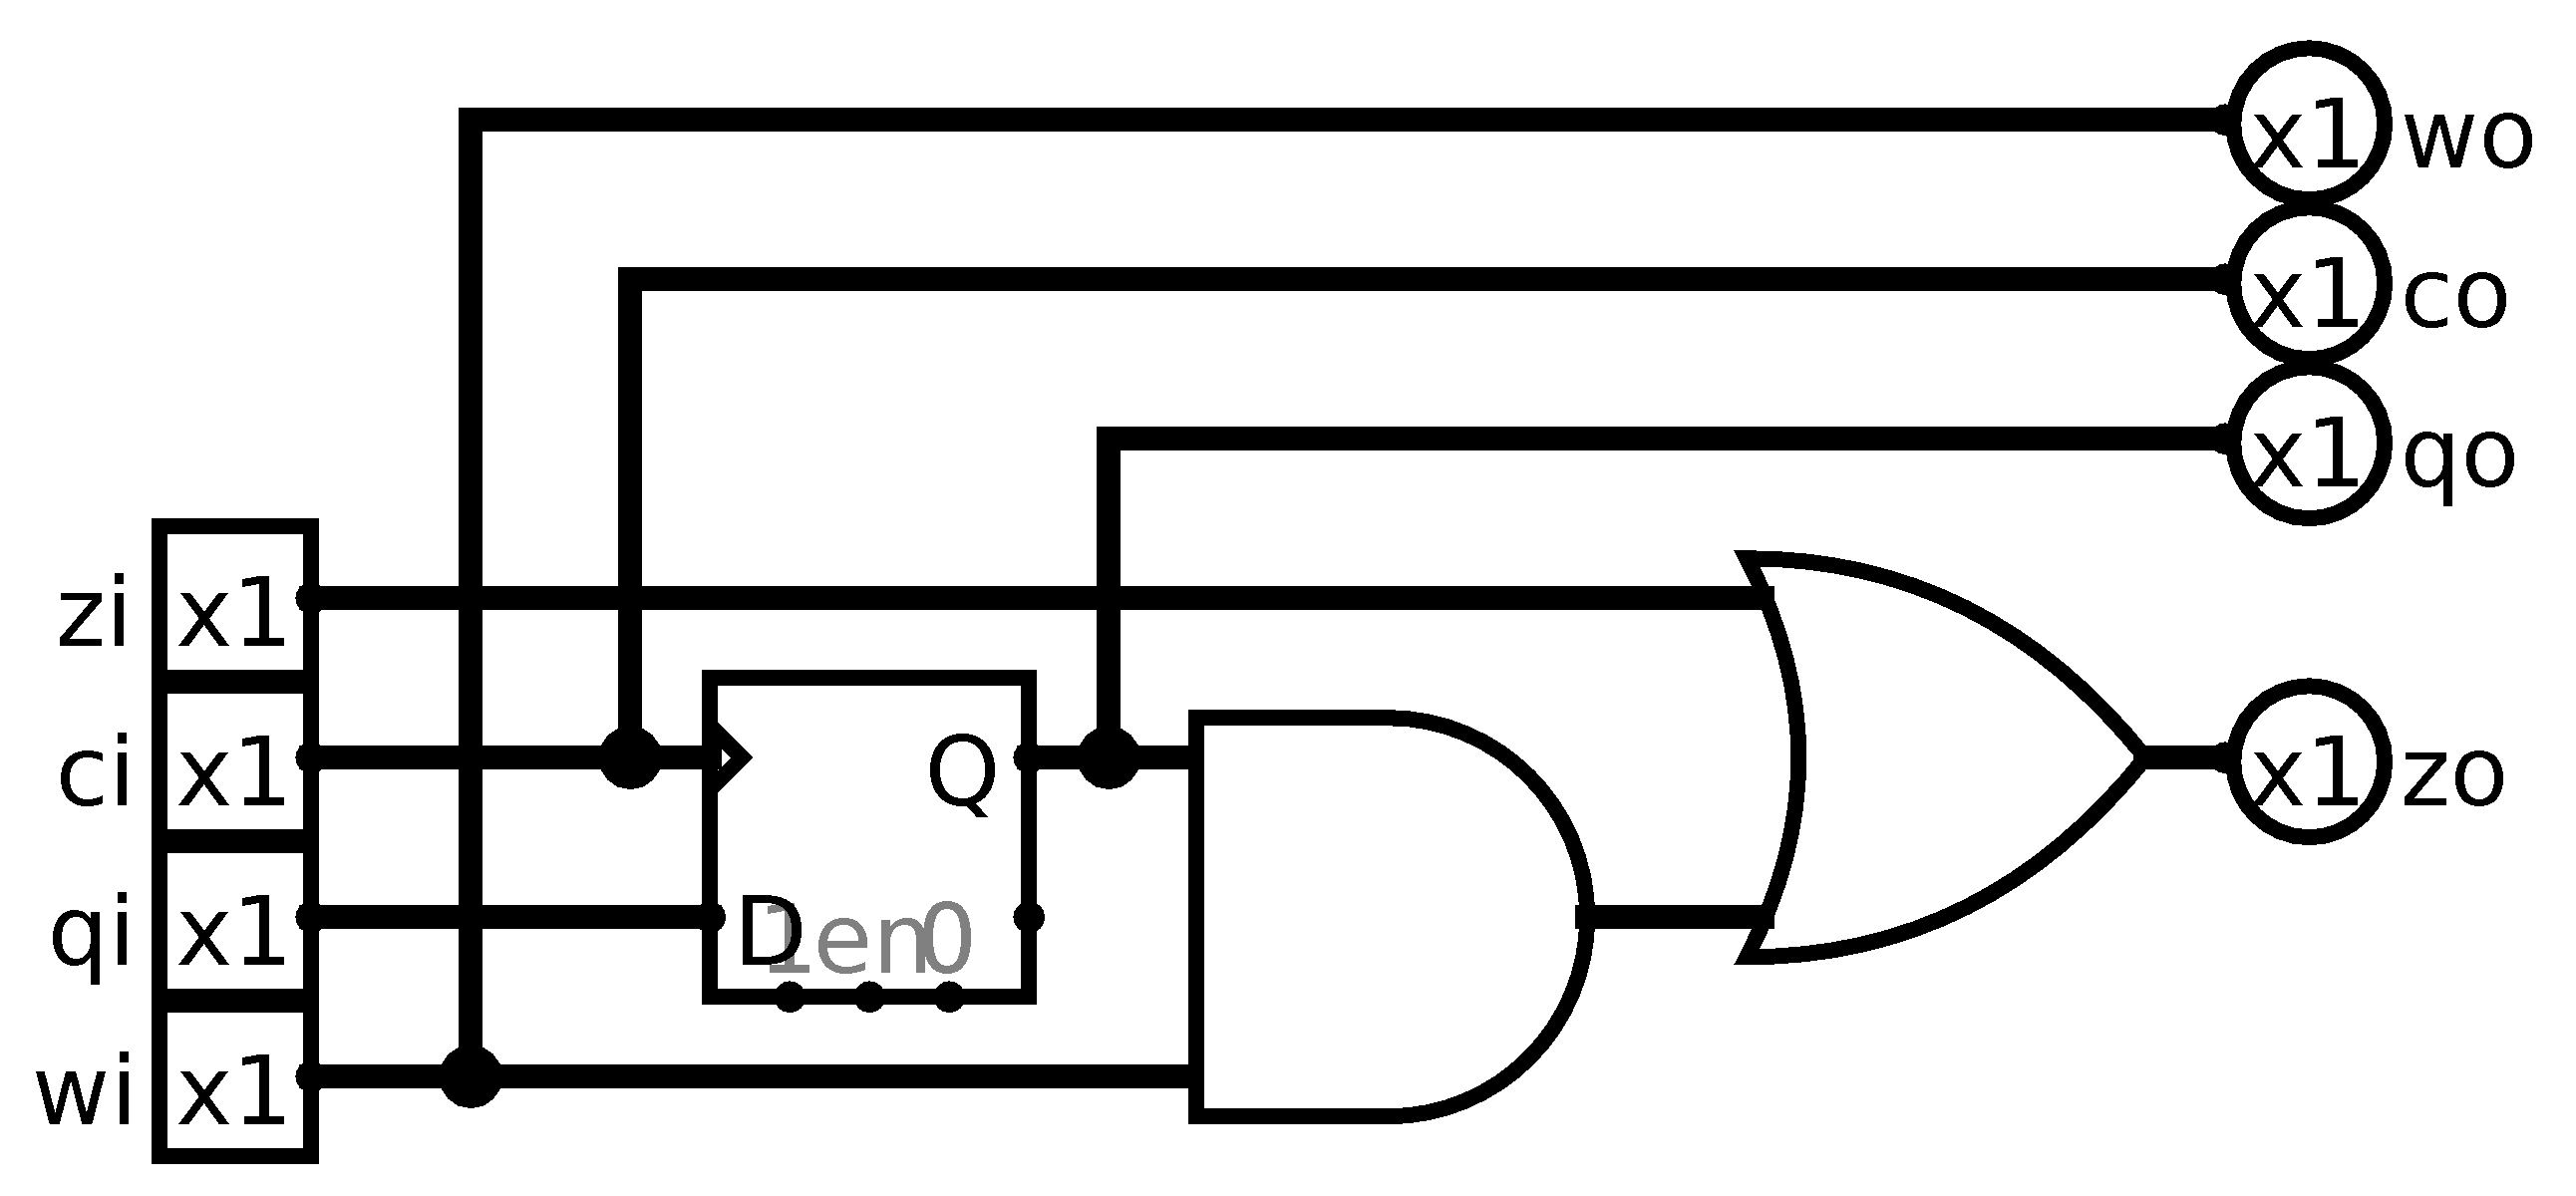
\includegraphics[width=0.75\linewidth]{../../logisim/pin_slice.png}
            \caption{Programmable Interconnect Network Bit-Slice}
        \end{figure}


\section{VHDL Models}
    \subsection{Top Level}
        \lstinputlisting[caption=Top Level VHDL Module]{../../vhdl/top.vhd}
        \begin{figure}[H]
            \centering
            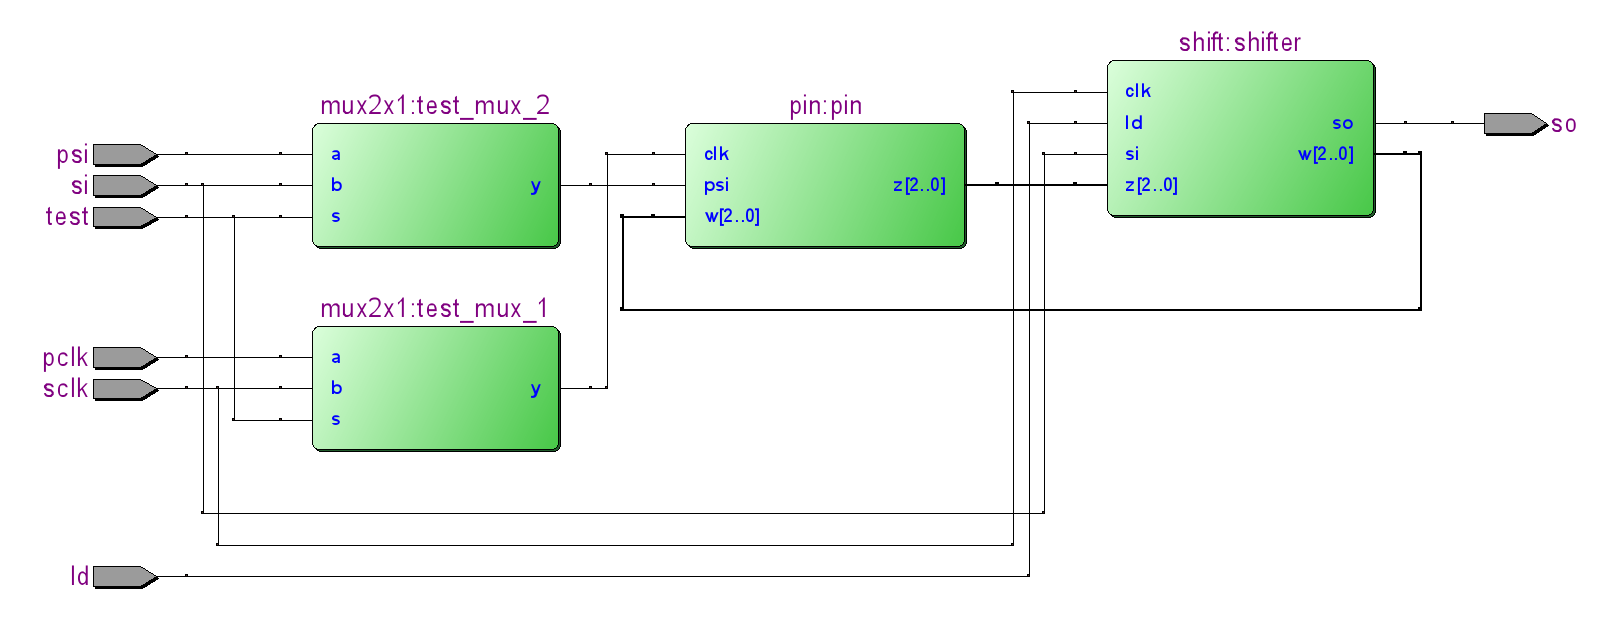
\includegraphics[width=\linewidth]{../../doc/rtl_pics/top_rtl.png}
            \caption{Top Level Generated RTL Diagram}
        \end{figure}
    \subsection{PIN}
        \lstinputlisting[caption=PIN VHDL Module]{../../vhdl/pin.vhd}
        \begin{figure}[H]
            \centering
            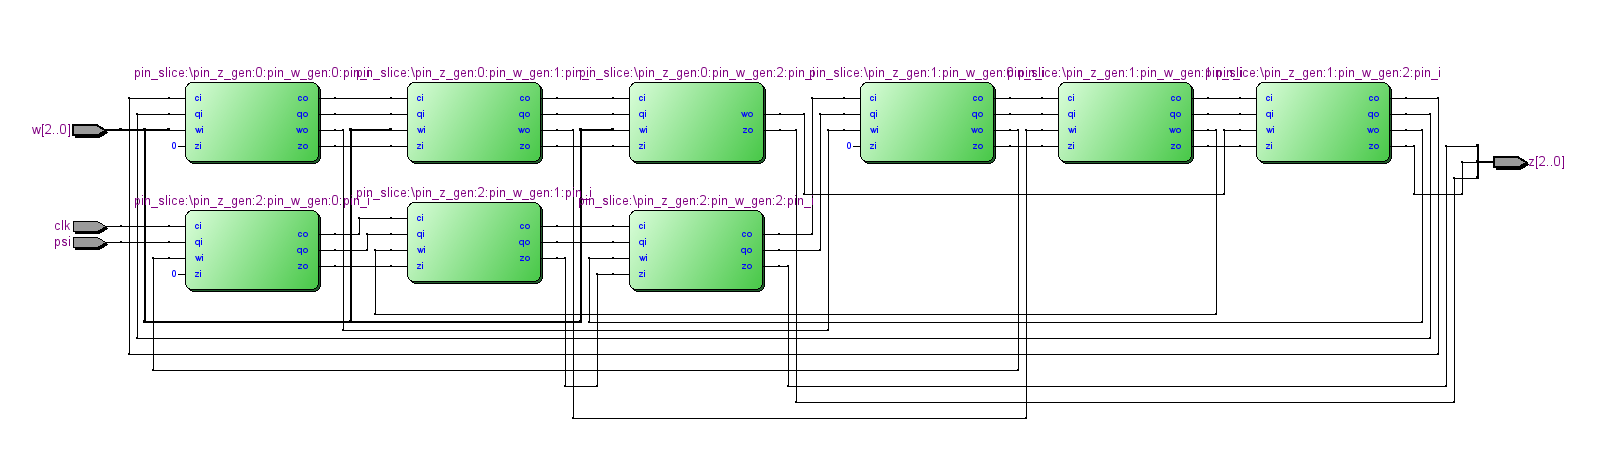
\includegraphics[width=0.5\linewidth]{../../doc/rtl_pics/pin_rtl.png}
            \caption{Pin Generated RTL Diagram}
        \end{figure}
    \subsection{PIN Slice}
        \lstinputlisting[caption=PIN Slice VHDL Module]{../../vhdl/pin_slice.vhd}
        \begin{figure}[H]
            \centering
            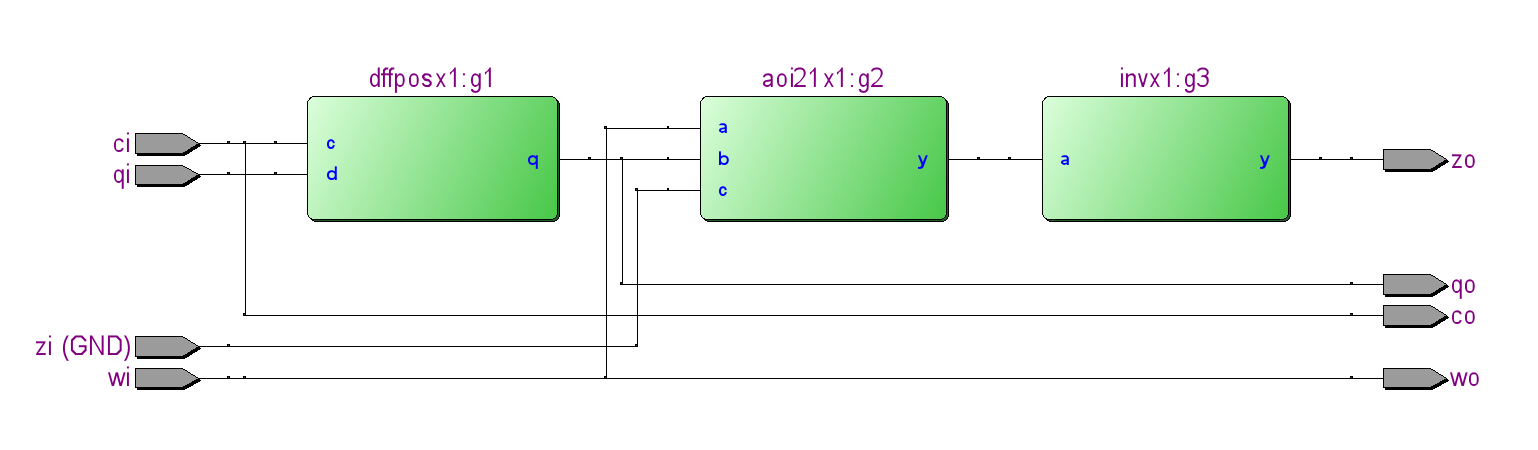
\includegraphics[width=\linewidth]{../../doc/rtl_pics/pin_slice_rtl.png}
            \caption{Pin Slice Generated RTL Diagram}
        \end{figure}
    \newpage
    \subsection{Shifter}
        \lstinputlisting[caption=Parallel Load Shifter VHDL Module]{../../vhdl/shift.vhd}
        \begin{figure}[H]
            \centering
            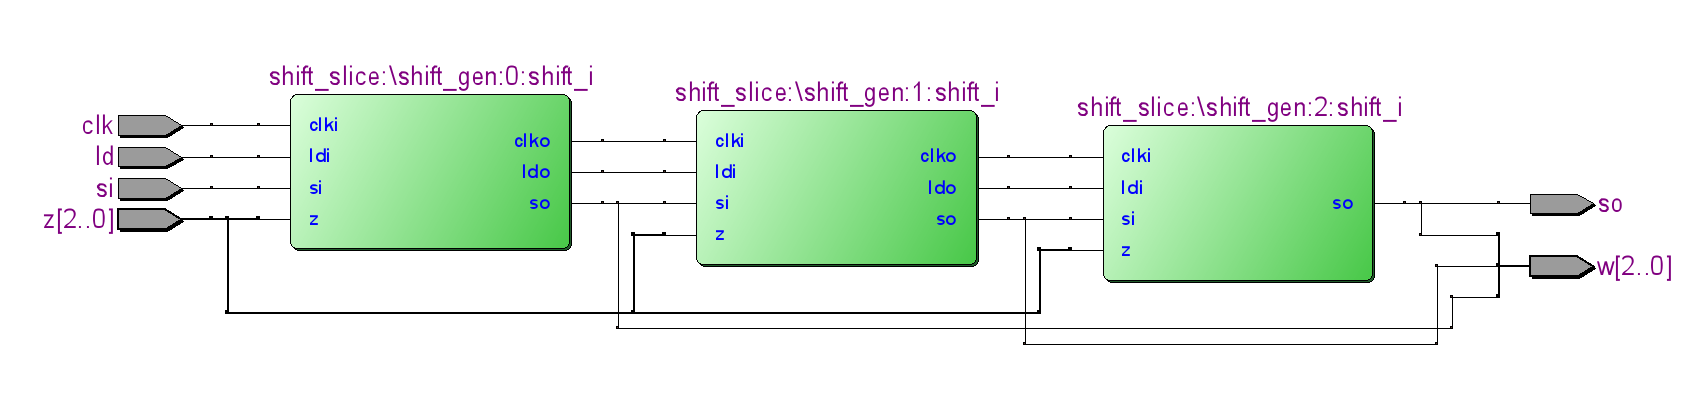
\includegraphics[width=\linewidth]{../../doc/rtl_pics/shift_rtl.png}
            \caption{Shifter Generated RTL Diagram}
        \end{figure}
    \newpage
    \subsection{Shifter Slice}
        \lstinputlisting[caption=Parallel Load Shifter Slice VHDL Module]{../../vhdl/shift_slice.vhd}
        \begin{figure}[H]
            \centering
            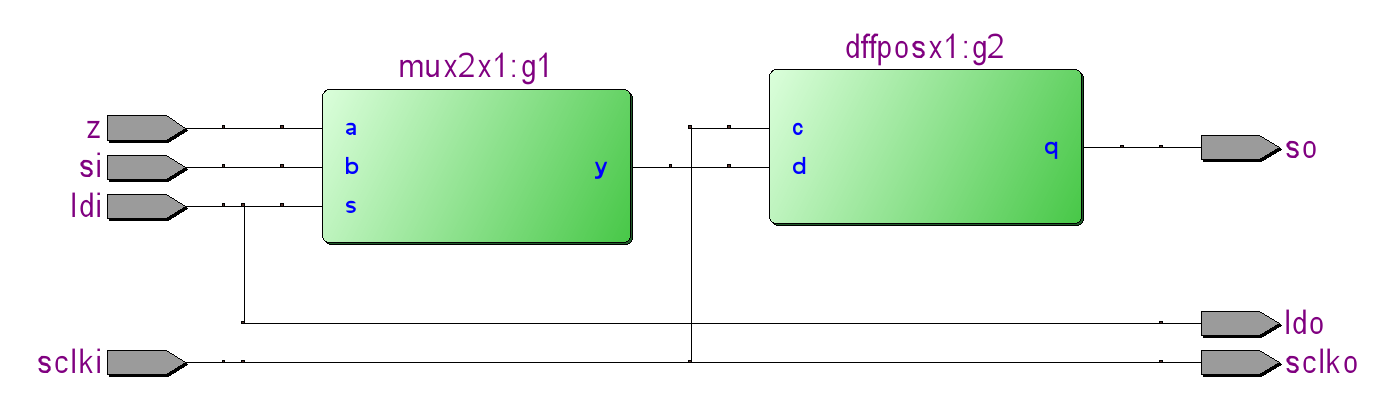
\includegraphics[width=\linewidth]{../../doc/rtl_pics/shift_slice_rtl.png}
            \caption{Shifter Slice Generated RTL Diagram}
        \end{figure}
    \newpage
    \subsection{Gates}
        \lstinputlisting[caption=AOI21X1 VHDL Module]{../../vhdl/aoi21x1.vhd}
        \lstinputlisting[caption=DFFPOSX1 VHDL Module]{../../vhdl/dffposx1.vhd}
        \lstinputlisting[caption=INVX1 VHDL Module]{../../vhdl/invx1.vhd}
        \lstinputlisting[caption=MUX2X1 VHDL Module]{../../vhdl/mux2x1.vhd}

\section{VHDL Test Benches}
    \subsection{Top Level Functional}
        \lstinputlisting[caption=Top Level VHDL Test Bench]{../../vhdl/top_tb.vhd}
        We decided to write a small Python script to generate the expected
        output vector for all possible PIN configurations and input values. Our
        test bench then runs through all of these vectors and checks if the
        output vector from our design matches the known output. If then
        indicates if they pass or fail.
        \lstinputlisting[caption=Python Vector Generator, language=Python]{../../vhdl/gen_sim.py}
    \newpage
    \subsection{Top Level Test Mode}
        \lstinputlisting[caption=Top Level Test Mode VHDL Test Bench]{../../vhdl/top_test_tb.vhd}
    %\subsection{PIN}
    \subsection{PIN Slice}
        \lstinputlisting[caption=PIN Slice VHDL Test Bench]{../../vhdl/pin_slice_tb.vhd}
    %\subsection{Shifter}
    \subsection{Shifter Slice}
        \lstinputlisting[caption=Parallel Load Shifter Slice VHDL Test Bench]{../../vhdl/shift_slice_tb.vhd}

\section{VHDL Test Bench Results}
    \subsection{Top Level Functional}
        While our top level functional testbench is completely automated and
        does an exhaustive test on all possible inputs an example waveform is
        shown below. We can first see that we clock in a PIN configuration
        vector of \texttt{000001000} which enables slice \texttt{Z1W2}. We then
        shift in a value of \texttt{001}. Given these input vectors we expect
        the output vector to be \texttt{010}. We can see from the waveform
        below that we achieve the expected result.
        \begin{figure}[H]
            \centering
            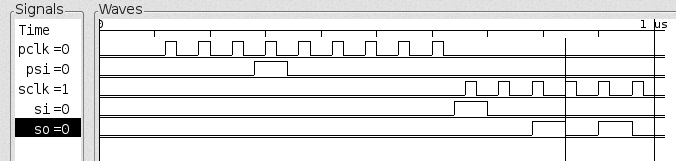
\includegraphics[width=\linewidth]{../../doc/vhdl_sim_pics/top.png}
            \caption{Top Level Functional Test Bench Waveform}
        \end{figure}
    \subsection{Top Level Test Mode}
        Our top level test mode testbench is also completely automated. For
        this test we simply send a pulse through all the flip flops and count
        the number of clock cycles it takes for the pulse to come out the other
        end. For a 3-Bit configuration there are 3*3+3 flip flops so we expect
        the pulse to appear at the output after 12 clock pulses. We can see
        from the waveform below that we achieve the expected output.
        \begin{figure}[H]
            \centering
            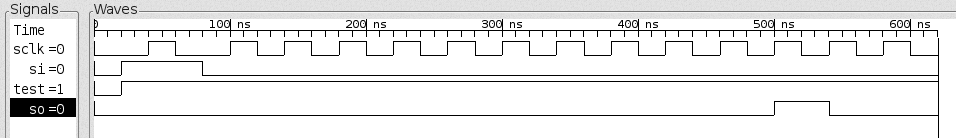
\includegraphics[width=\linewidth]{../../doc/vhdl_sim_pics/top_test.png}
            \caption{Top Level Test Mode Test Bench Waveform}
        \end{figure}

\section{Work Division}

\begin{table}[H]
    \centering
    \begin{tabular}{ll}
        \toprule
        \textbf{Task} & \textbf{Person}\\
        \midrule
        Pinout Diagram & Both \\
        Explanation of Functionality & Both \\
        Design Decisions & Both \\
        Top Level Block Diagrams & Both \\
        Shifter Block Diagrams & Qi \\
        PIN Block Diagrams & Thrun \\
        VHDL Shifter+TB & Qi \\
        VHDL PIN+TB & Thrun \\
        VHDL Top+TB & Both \\
        VHDL Top Test Mode TB & Thrun \\
        \bottomrule
    \end{tabular}
    \caption{Task Assignment}
\end{table}

\end{document}
